\section{\linkeddata}
Actualmente se está ante un entorno de datos fluyendo constantemente, esperando a ser utilizados para generar información
sobre un determinado acontecimiento. De esta manera, podemos ser conscientes de las últimas noticias, productos de una determinada
marca o simplemente sobre información de nuestros contactos en las redes sociales. Esta nueva situación implica que existe un nuevo
mercado para la construcción de aplicaciones y servicios~\cite{Krafzig2004} que exploten estos datos, generando nuevos negocios~\cite{web20} y conectando a las comunidades
científicas, y en general fomentando el progreso de una forma sostenible. Por ejemplo, algunos servicios de búsqueda como Google~\cite{Google} utilizan los
datos publicados en las tiendas de Internet como Amazon~\cite{Amazon}, para extender y procurar resultados de búsqueda más ajustados. En esta línea, prestando 
atención a los resultados de los principales buscadores, las primeras sugerencias corresponden a páginas de Wikipedia~\cite{Wikipedia}, Facebook~\cite{Facebook},
 Linkedin~\cite{Linkedin}, etc.,  por lo que efectivamente queda patente que los servicios de búsqueda~\cite{Pound}, entre otros, están sacando partido de los datos estructurados publicados en distintos sitios web, para así identificar descripciones, organizaciones, personas, perfiles profesionales o productos y 
ofrecer resultados más acordes con la intención de los usuarios.

La evolución hacia esta nueva web, también de denominada Web $3.0$, globalmente enlazada mediante datos supone una transición~\cite{Ankolekar07thetwo}
de la web tradicional orientada a documentos (Web $1.0$) y dirigida hacia las personas principalmente, incluyendo relaciones (Web $2.0$),
a una nueva \wode, en la cual los datos se publican para ser tratados tanto por los humanos como
por los agentes automáticos, proporcionando descripciones más completas a todos los niveles. En este
sentido, \textit{Tim Berners-Lee} explica convenientemente los principios de esta nueva web realizando una analogía 
de una bolsa de patatas~\cite{TBL-crisps} con una página web, en la cual la parte delantera estaría orientada 
hacia las personas, mientas que la información (meta información) de la parte trasera serían datos
dirigidos hacia otros agentes.

Actualmente la publicación de datos se haya envuelta en distintos dominios en los que previamente
nunca se había pensado compartir datos, pero en los que se están generando nuevos servicios y 
oportunidades de negocio a partir de esta iniciativa que busca la compartición de datos. En 
este estado pueden surgir varias preguntas:
\begin{itemize}
 \item ¿Cómo se deben publicar los datos para ser reutilizados?
\item ¿Existen mecanismos para la reutilización automática?
\item ¿Cuál es la forma más ágil para integrar fuentes de datos heterogéneas?
\item ¿Se puede asegurar la calidad de los datos en términos de disponibilidad, autenticidad, evolución, etc.?
\end{itemize}

Estamos, en consecuencia, ante una revolución del uso de datos en la Web, entorno en el cual se pueden realizar
diferentes operaciones sobre los mismos: descubrimiento, consulta, integración y explotación. La Web ofrece
su infraestructura~\cite{webarch}, protocolos y amplio asentamiento para reducir el impacto de esta evolución. No obstante, esta nuevo 
entorno trae consigo nuevos requisitos arquitectónicos, necesidad de entender el comportamiento de las \gls{URI}s~\cite{uri-rfc} y del 
protocolo \gls{HTTP}~\cite{http-rfc} para reutilizar la infraestructura existente y concienciar a la comunidad del empleo de este entorno. 

\subsection{Definición y necesidad de \textit{Linked Data}}\label{def-linkeddata}
\textit{Tim Berners-Lee} acuñó esta iniciativa en el año 2006~\cite{Berners-Lee-2006} como parte de la Web Semántica~\cite{Berners-Lee2001,WeavingTim,berners-lee06a}. 
En un principio la Web Semántica surgió con el objetivo de integrar grandes bases de datos a través de modelos de conocimiento compartidos u ontologías, de esta manera
cualquiera podría reutilizar el conocimiento ya consensuado y en consecuencia los datos asociados a esta información. Si bien
la Web Semántica tuvo un gran éxito desde un punto de vista teórico, en la práctica escasas aplicaciones reales llegaron a tener
un notable impacto en el gran público~\cite{sw-use-cases}. Es por ello, que tomando la visión de la Web Semántica en su parte de modelos y formatos de datos
estandarizados formalizados a través de conocimiento compartido, fue tomada para definir lo que actualmente se conoce como \linkeddata~\cite{linked-data}.
En realidad se trata de un enfoque práctico de la Web Semántica, en el cual
se hace uso de los fundamentos de la semántica y de la web para proveer mecanismos para la publicación~\cite{bizer07how,Berr08} y 
consumo de datos masivos sin tener grandes barreras de entrada y claramente orientado al desarrollo de aplicaciones. 
Análogamente en el arranque de la web orientada a documentos se realizó un esfuerzo para identificar cómo publicar documentos, por ejemplo utilizando HTML, pero no se hizo hincapié en
modelar la información que se publicaba en los mismos, esto ocasionó que la Web que hoy conocemos despegara exponencialmente. En el caso
de la \wode se realiza un enfoque similar, es decir, se establece cómo publicar datos, sin embargo no presta especial énfasis
 en que estos datos estén formalizados estrictamente sobre un modelo conocimiento. De esta manera se facilita y favorece el crecimiento y la aparición de nuevas fuentes
de datos en la Web. No obstante, esta segunda parte de modelado y estructuración de datos deviene fundamental para ciertas tareas
automáticas.

El objetivo por lo tanto de la \wode no se centra tan sólo en publicar datos sino en hacer los datos accesibles, tanto a las personas
como a las máquinas, como son actualmente los documentos disponibles en la Web. La diferencia sustancial reside en que actualmente
la web está orientada al uso por personas y las máquinas necesitan procesos dotados de un cierto grado de complejidad para acceder a esta información.
Por lo tanto, con esta nueva iniciativa se facilitan los enlaces entre los datos para que puedan ser explorados eficientemente 
por cualquier agente y realizar operaciones de enriquecimiento y enlazado de forma sencilla.

La \wode se construye sobre enlaces como la web tradicional en la que los documentos son enlazados entre sí. La diferencia
reside en que los datos utilizan enlaces en \gls{RDF} para describir recursos de distintos tipos identificados de forma unívoca
mediante un \gls{URI} y siguiendo unos principios que, aunque analizados en detalle en la Sección~\ref{principos-linked-data}, se presenta a continuación una breve descripción de los mismos:
\begin{itemize}
 \item \textit{Use URIs as names for things}. Utilizar URIs como nombres para identificar y acceder a los recursos.
 \item \textit{When someone looks up a URI, provide useful information, using the standards (RDF*, \gls{SPARQL}~\cite{Sparql})}. El acceso 
a los recursos a través de URIs debe estar basado en estándares como RDF o SPARQL suministrando igualmente información
sobre el acceso.
\item \textit{Include links to other URIs. so that they can discover more things}. Enlazar datos no sólo implica la publicación
masiva de datos sino que se deben establecer enlaces entre ellos con el objetivo de proveer un entorno navegable~\cite{Berners-lee06tabulator:exploring,Pietriga06fresnel}.
\item \textit{Use \gls{HTTP URI}s so that people can look up those names}. Utilizar URIs HTTP para reaprovechar la actual infraestructura
de la web y que el público potencial pueda acceder a los datos de la misma forma que se realiza en el presente con los documentos.
\end{itemize}

En este contexto formalizado con reglas muy explícitas, queda patente 
que uno de los factores clave de esta iniciativa reside en poder de reutilizar información bien 
estructurada desde la propia fuente de datos, facilitando así la creación de aplicaciones fiables en el 
sentido del tratamiento de datos y evitando el uso de otras técnicas basadas en estadística y procesamiento
de lenguaje natural, que se siguen aplicando ya que no siempre se cumple con todos los requisitos que establece la iniciativa de \linkeddata.

En resumen, el objetivo de la iniciativa de \linkeddata es enlazar datos de fuentes heterogéneas entre sí, 
con el objetivo de enriquecer la información y ofrecer a todos los agentes tanto personas como máquinas
un espacio homogéneo basado en estándares para la realización de las operaciones citadas anteriormente, descubrimiento, acceso y explotación. 
Para ello se hace uso de la tecnología semántica \gls{RDF} que provee una forma flexible y escalable para la realización de descripciones de las entidades 
del mundo: personas, organizaciones, localizaciones, etc. Las sentencias en RDF permiten
establecer de una forma sencilla enlaces entre ellas creando conexiones desde un entorno local
hacia un entorno global. También cabe destacar que el uso de RDF difiere de los actuales
documentos presentes en la web en dos puntos importantes:

\begin{itemize}
 \item El enlace se produce a nivel de entidades, no de documentos.
 \item Cada enlace tiene un tipo definido.
\end{itemize}

\linkeddata permite así establecer conexiones entre diferentes fuentes de datos y crear un espacio 
de datos global, esto es posible gracias al uso de estándares y de un modelo de datos común que facilita
la creación de aplicaciones de carácter general capaces de operar en este nuevo espacio de datos.

El gran valor de \linkeddata se centra por tanto en brindar una oportunidad para utilizar los datos
y explotar su valor mediante sistemas basados en conocimiento, con capacidad de procesar una cantidad
masiva de datos obteniendo así soluciones más fiables y aproximadas a las necesidades y expectativas
de los agentes. En síntesis, ver Tabla~\ref{tabla:linked-data}, se pueden establecer una serie de características y criterios a satisfacer.

\begin{longtable}[c]{|l|p{7cm}|p{7cm}|} 
\hline
  \textbf{ID} & \textbf{Directriz} &  \textbf{Descripción} \\\hline
\endhead
   \multicolumn{3}{|c|}{\textbf{Principios Linked Data}}  \\ \hline
   1.1&\textit{Use URIs as names for things} & \\ \hline
   1.2&\textit{When someone looks up a URI, provide useful information, using the standards (RDF*, SPARQL)} & \\ \hline  
   1.3&\textit{Include links to other URIs} & \\ \hline    
   1.4&\textit{Use HTTP URIs} & \\ \hline    
  \multicolumn{3}{|c|}{\textbf{Modelo $\star$}}  \\ \hline
     2.1&$\star$	& \textit{Available on the web (whatever format) but with an open licence, to be \opendata} \\ \hline 

2.2&$\star \star$	 &  \textit{Available as machine-readable structured data (e.g. excel instead of image scan of a table)} \\ \hline 

2.3&$\star \star \star$	&  \textit{ as (2) plus non-proprietary format (e.g. \gls{CSV} instead of exce}l) \\ \hline 

2.4&$\star \star \star \star$	&  \textit{All the above plus, Use open standards from \gls{W3C} (RDF and SPARQL) to identify things, so that people can point at your stuff} \\ \hline 
 
2.5&$\star \star \star \star \star$	 & \textit{All the above, plus: Link your data to other people’s data to provide context}                                     \\ \hline 
  \hline
  \caption{Características a tener en cuenta sobre \linkeddata.}
  \label{tabla:linked-data}
\end{longtable}

\subsection{\opendata}\label{opendata-sect}
Este término se enclava dentro de las definiciones de conocimiento abierto realizadas por
la organización \textit{Open Knowledge Foundation}~\cite{okfn} (\gls{OKFN}), en el cual también se incluyen:
\begin{itemize}
 \item Contenidos como libros, películas, música y cualquier otro material con autoría definida.
\item Datos, en general, pertenecientes a distintos contextos: científicos, históricos o geográficos.
\item Información proveniente de las Administraciones Públicas.
\end{itemize}

Siguiendo la definición realizada por esta institución, cuando una obra o datos satisfagan las siguientes
condiciones serán consideradas como abiertas:

\begin{description}
 \item [Acceso.] La obra debe estar disponible íntegramente y sólo a un coste de 
  reproducción razonable, preferiblemente para su descarga de modo gratuito en Internet. 
  La obra también debe estar disponible en una forma conveniente para ejecutar modificaciones sobre ella.
 \item [Redistribución.] La licencia no debe contener restricciones sobre la posibilidad de venta o 
  distribución de la obra en sí misma o formando parte de un paquete constituido por obras de fuentes diversas. 
  La licencia no debe exigir un pago u otro tipo de cuota para esta venta o distribución.
 \item [Reutilización.] La licencia debe permitir hacer modificaciones y obras derivadas facultando que éstas sean distribuidas en las mismas condiciones que la obra original. La licencia puede imponer algún tipo de requisito relativo al 
  reconocimiento y a la integridad: veáse el principio 5 (Reconocimiento) y el principio 6 (Integridad) reseñados más adelante.
 \item [Ausencia de restricciones tecnológicas.] Se debe proporcionar la obra de modo que no presente ningún obstáculo tecnológico para ejecutar los actos mencionados anteriormente. Esto se puede conseguir ofreciendo la obra en un formato de datos abierto, por ejemplo un formato cuya especificación esté disponible públicamente y de manera gratuita, de modo que para su uso no se imponga ninguna restricción de tipo monetario o análogas.
 \item [Reconocimiento.] La licencia puede exigir como condición para la redistribución y la reutilización el reconocimiento de los contribuyentes y creadores de la obra. Si se impone esta condición, no debe ser de manera onerosa. Por ejemplo si se exige un reconocimiento, la obra debería ir acompañada de una lista de aquellos susceptibles del mismo.
 \item [Sin discriminación de personas o grupos.] La licencia no debe discriminar a ninguna persona o grupo de personas.
 \item [Sin discriminación de ámbitos de trabajo.] La licencia no debe contener restricciones sobre el uso en un ámbito de trabajo específico. Por ejemplo, no se puede limitar el uso de la obra en un negocio, o que ésta sea utilizada para investigación militar.
 \item [Distribución de la licencia.] Los derechos adjuntos a la obra deben aplicarse también a todo áquel a quien le sea redistribuida, sin necesidad de que éste disponga una licencia adicional.
 \item [La licencia no debe ser específica de un paquete.] Los derechos adjuntos a la obra no deben depender de que la obra forme parte de un paquete particular. Si la obra se extrae de ese paquete y se utiliza o se distribuye en las condiciones de la licencia de la obra, todos aquellos a quien les sea redistribuida deberán tener los mismos derechos que los concedidos conjuntamente con el paquete original.
 \item [La licencia no debe restringir la distribución de otras obras.] La licencia no debe imponer restricciones en otras obras distribuidas conjuntamente con la obra objeto de la licencia. Por ejemplo, la licencia no debe imponer que todas las otras obras que se distribuyan por el mismo medio sean abiertas.
\end{description}

La corriente de datos abiertos~\cite{odfn} ha sido especialmente acogida en el ámbito de las Administraciones
Públicas, ver Figura~\ref{fig:od-spain}, adaptando las directrices aquí fijadas para desplegar el movimiento
de \ogd. 

\begin{figure}[!htb]
\centering
	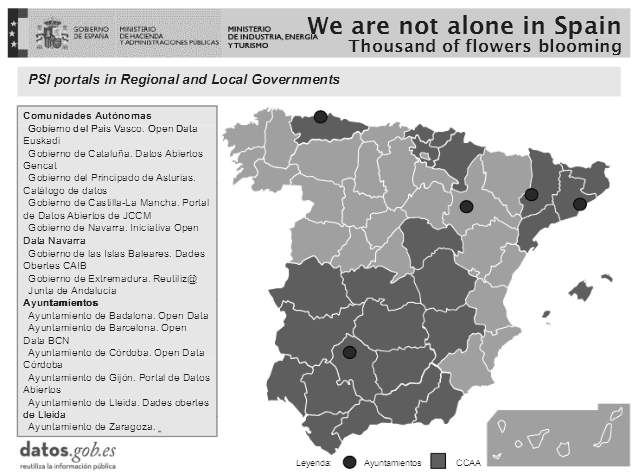
\includegraphics[width=14cm]{images/phd/open-data-spain}
\caption{Estado de \opendata en España por el Ministerio de Hacienda y Administraciones Públicas}
\label{fig:od-spain}
\end{figure}

Las instituciones públicas han establecido distintos canales de comunicación~\cite{improvingW3c}
con los ciudadanos, intentando siempre mejorar la interacción en los distintos
procesos administrativos. Por ello y para estar presentes en las principales iniciativas
de comunicación han procurado atender a los avances tecnológicos. Desde
principios de la década de los años noventa han tenido presencia en la web proveyendo
distintos servicios para que el ciudadano pueda agilizar sus trámites
y así obtener una administración más eficiente, tanto en tiempo como en uso
de recursos. Esta situación ha derivado a lo que se denomina como ``administración
electrónica'' o \egov, en la cual la información de los servicios
y datos que obran en poder de la Administración resultan de fácil acceso a los
 ciudadanos a través de los principales canales de comunicación, 
como la web, dispositivos móviles, etc., creando de esta forma
una administración con una ventanilla única, fijando como objetivo principal
 la transparencia y la objetividad, materializadas a través de distintas
políticas, concretamente en el caso europeo se dispone de un Plan de Acción~\cite{policy-eu} específico para el período 2011-2015.

No obstante, aunque las intenciones están acertadamente fijadas existen muchos
desafíos que han estado y están impidiendo el despegue definitivo de la administración
electrónica, desde la tecnología hasta el necesario cambio tanto para los
integrantes de la propia administración como para los ciudadanos. Proveer
servicios y datos a través de la red se ha convertido en un desafío en el cual 
se encuentran inmersas las distintas administraciones, esta situación
implica ejecutar una gran inversión para dar cabida a todas las necesidades desde un punto
de vista tanto en materia de infraestructura como de concienciación social. De esta forma,
un gobierno basado en administración electrónica debe ser capaz de fijar los requisitos
de los servicios y datos a liberar, asegurar la autenticidad y definir la legislación
pertinente que establezca un marco jurídico seguro para que los ciudadanos pueden utilizar
toda la información disponible para consultar o construir nuevos servicios de valor
añadido sobre ellos.

Entre las actividades que se presentan como clave para el desarrollo de la administración
electrónica se pueden referir las siguientes:
\begin{itemize}
 \item Uso y aplicación de estándares.
 \item Transparencia y participación.
 \item Concienciación de los avances en la gestión e integración de datos.
 \item Relaciones y colaboraciones.
\end{itemize}

En este contexto se determinan por una parte los objetivos de la administración
respecto a disponer un entorno flexible y dinámico para sus ciudadanos, y por otra parte 
se encuentra el comportamiento de las propias personas y organizaciones. Actualmente
se advierte un entorno definido por las siguientes características: 
global, conectado, cambiante y accesible en su mayor parte.

El término de \ogd ha sido designado en la administración de Estados Unidos para indicar
aquellos datos o registros de información que obran en poder de la Administración Pública y que
han sido recabados con distintos objetivos en los distintos procesos administrativos. Como ejemplos
de reutilización en el sector público se encuentran los siguientes dominios: salud, cartografía, datos
meteorológicos, educación, datos bibliográficos, contratación pública, legislación, etc. Como 
se ha comentado con carácter previo, las organizaciones públicas producen, almacenan y distribuyen distintos tipos
de información: legal, financiera, geográfica, etc., en su actividad diaria. Esta información
proveniente del sector público (\gls{PSI}) está enclavada dentro de un marco jurídico que puede variar de un país a otro, 
por ejemplo en Europa la Directiva 2003/98/EC~\cite{d2003,d2003-update}, en España la Ley 37/2007~\cite{l37-2007} y su Real Decreto 1495/2011~\cite{r-1495} 
de desarrollo, Reino Unido~\cite{uk2012}, Francia~\cite{fr2012} o la iniciativa de la Casa Blanca en Estados Unidos~\cite{usa}. 
Habitualmente se utilizaban distintas técnicas y formatos
para la distribución de la información del sector público por diferentes canales desde el papel y correo postal, hasta
formatos electrónicos y las propias páginas web. La evolución en los últimos
años ha sido de gran calado de modo que ha hecho necesario dictar una legislación común que 
debe ser transpuesta en los diferentes países, como ocurre en el caso de Europa.

La transición hacia este nuevo enfoque administrativo todavía se encuentra
en una etapa temprana debido a las dificultades que supone toda una nueva forma de
actuar. En general, se suele hablar de \gd y \pusi para referirse al mismo concepto. Se han realizado diferentes definiciones como las
presentes en la iniciativa \ogd, pero no sólo se trata de exponer de forma pública 
las grandes bases de datos gubernamentales, sino que éstas deberían cumplir 
unos principios~\cite{8-principles} que a continuación se listan:

\begin{enumerate}
 \item Data Must Be \textit{Complete}. \textit{All public data are made available. Data are electronically stored information or recordings, including but not limited to documents, databases, transcripts, and audio/visual recordings. Public data are data that are not subject to valid privacy, security or privilege limitations, as governed by other statutes.}
 \item Data Must Be \textit{Primary}. \textit{Data are published as collected at the source, with the finest possible level of granularity, not in aggregate or modified forms.}
 \item Data Must Be \textit{Timely}. \textit{Data are made available as quickly as necessary to preserve the value of the data.}
 \item Data Must Be \textit{Accessible}. \textit{Data are available to the widest range of users for the widest range of purposes.}
 \item Data Must Be \textit{Machine processable}. \textit{Data are reasonably structured to allow automated processing of it.}
 \item Access Must Be \textit{Non-Discriminatory}. \textit{Data are available to anyone, with no requirement of registration.}
 \item Data Formats Must Be \textit{Non-Proprietary}. \textit{Data are available in a format over which no entity has exclusive control.}
 \item Data Must Be \textit{License-free}. \textit{Data are not subject to any copyright, patent, trademark or trade secret regulation. Reasonable privacy, security and privilege restrictions may be allowed as governed by other statutes.}
\end{enumerate}

Con todo ello, se provee un entorno en el cual ``público'' designa a las condiciones que deben cumplir los datos
para considerarse ``abiertos'', no se entra a valorar los datos que se deben liberar ni tampoco cuestiones
legales. En cuanto a los ``datos'', se toma este término para designar a los registros electrónicos, es importante
destacar que los documentos físicos no se consideran como tal, que obran en poder de la administración y finalmente,
con ``revisable'' se denomina a aquellos datos para los cuales existe una persona de contacto que actúa como
enlace para aquellos que quieran usar los datos, para gestionar el uso de los mismos y para los que 
existe un órgano administrativo o judicial que posee la potestad para aplicar adecuadamente los principios citados.

Por otra parte, existen cuestiones~\cite{publishing-ogd} que deben tener respuesta en el contexto de \ogd desde un punto
de vista estratégico hasta funcional, como qué tipo de interfaz de acceso (\gls{API}) se debe proveer para el acceso a los datos, por ejemplo, 
en cuanto a los datos a liberar, la iniciativa de datos abiertos no especifica qué datos deberían liberarse. Corresponde
a la estrategia del organismo en cuestión establecer las prioridades, coste y beneficios de la liberación de un determinado conjunto
de datos. En determinados casos como el del Gobierno de Reino Unido~\cite{uk-survey} o el Ayuntamiento de Zaragoza~\cite{zar-survey} se utilizan encuestas
a los propios usuarios para especificar o establecer un orden en los datos a liberar. El objetivo final será
disponer de una política y guías de apertura de datos que sean capaces de dar soporte a los siguientes puntos:

\begin{description}
 \item [Inclusión.] El uso de estándares facilita la accesibilidad y la usabilidad de los datos. De esta forma,
se facilita la participación de terceros y el desarrollo de aplicaciones de distinto carácter que beneficiarán
transversalmente a toda la sociedad con nuevos servicios.
\item [Transparencia.] En los últimos años y debido a los múltiples casos de corrupción a nivel político, deficiente gestión
de fondos públicos y en general, cierta falta de claridad por parte de las instituciones ha hecho que esta corriente 
sitúe como un eje el impulso de la transparencia en el conjunto de las Administraciones Públicas.
\item [Responsabilidad.] La eficiencia en el uso de recursos debe ser uno de los objetivos de la Administración Pública, por ello
conseguir información sobre su funcionamiento puede mejorar el mismo a nivel interno.
\end{description}

Una vez que se dispone de datos abiertos cabe definir cómo se pueden obtener mejoras en ciertos procesos de uso. Entre 
ellos se puede destacar:

\begin{description}
\item [Reutilizar.] La información abierta permite plantear nuevos modelos de interacción, tanto para otras administraciones públicas
como para organizaciones o comunidades que se beneficien de estos datos para el despliegue de nuevos servicios~\cite{web20}. Actualmente
se realizan actividades para el impulso de la reutilización de datos, como los concursos en los que liberados datos, los interesados 
presentan aplicaciones haciendo uso de ellos.
 \item [Generar múltiples vistas de los datos~\cite{DBLP:journals/semweb/DadzieR11}.] Cuando se dispone de los datos de una forma más o menos estandarizada y con facilidad
de acceso se pueden generar múltiples vistas, dependiendo de las necesidades del usuario y adaptándolos al contexto. Por ejemplo,
generación de informes en PDF, visualización en mapas de la información geográfica, etc. Partiendo de los mismos datos y en algunos
casos y tras la ejecución de un proceso de enriquecimiento se puede mejorar la información que provee. El coste de realización de 
estos procesos es alto si está centralizado en la administración, pero se puede diversificar y abaratar delegando en 
terceras partes.
 \item [Mejorar los actuales sistemas de búsqueda~\cite{hoga-etal-2011-swse-JWS}.] Un sistema de búsqueda dispondrá de mayor precisión cuanto más ``informado'' esté, por lo tanto,
si se pueden reutilizar los datos ya disponibles para mejorar los resultados de las consultas de los usuarios, se facilitará el acceso a la
información.
  \item [Integrar fuentes de datos~\cite{Andreas_Schultz_Isele_Bizer_Becker_2011,Harth:2011:SIP:1963192.1963318}.] Habitualmente cada organismo goza de cierta independencia para gestionar sus propios datos. La realidad
es que en muchos casos diferentes organismos de la misma entidad tienen la necesidad de cruzar datos para obtener diferente información
agregada. Si se utilizan datos abiertos se favorece la integración y la reutilización de datos disminuyendo los costes de la obtención
y gestión de los mismos al no estar multiplicada.
\end{description}

Una vez que se han definido algunos de los beneficios del uso de datos abiertos en el ámbito de las
administraciones públicas, cabe ahora especificar cómo han de ser publicados para que
puedan ser consumidos por terceros de forma ágil. Para ello se han establecido una serie
de directrices o métodos:
\begin{itemize}
 \item Usar anotaciones basadas en microformatos o \gls{RDFa}~\cite{rdfa-primer} en \gls{XHTML} o \gls{HTML}5~\cite{HTML5}.
 \item Facilitar la accesibilidad siguiendo las directrices \gls{WCAG}~\cite{wcag2}.
 \item Desplegar APIs específicas para el consumo de datos.
 \item Sindicar de contenidos mediante \gls{RSS}~\cite{rss} o \gls{ATOM}~\cite{atom-rfc}.
 \item Proveer interfaces \gls{REST}~\cite{Fielding2000} o \gls{SOAP}~\cite{SOAP11} de servicios de acceso a datos.
 \item Aplicar tecnologías semánticas mediante \gls{RDF}.
\end{itemize}

Finalmente se ha de definir la misión y estrategia de apertura de datos, así la confianza (\trust), procedencia~\cite{Carroll05namedgraphs,prov-group} (\provenance) y calidad de los mismos, la
evolución en tiempo, las limitaciones tecnológicas y la capacidad para seguir creciendo. De acuerdo a lo expuesto en esta sección se pueden
establecer una serie de factores a evaluar sobre la publicación de datos abiertos de acuerdo a distintos criterios y que 
servirán para comprobar si se cumplen las guías definidas. 

\subsection{\lod}
La convergencia entre las iniciativas de \linkeddata y \opendata ha conllevado la creación
de un nuevo término para designar a aquellos datos que cumplen las guías de ambas iniciativas y que 
se denomina \lod. Bajo esta definición se agrupan todos los datos que han sido
liberados aplicando los principios de \linkeddata y que además cumplen significativamente
las directrices de \opendata. Habitualmente este término se aplica en el contexto de las Administraciones
Públicas, en las que el esfuerzo por la apertura de datos ha sido intenso y en el que han logrado grandes avances. 

El alto valor de los datos enlazados abiertos permite disfrutar a terceros de la posibilidad real 
de creación de servicios de alto valor añadido. No obstante, surge la duda de si el proceso de enlazado de datos
y de explotación, corresponde a la propia Administración o si cabe delegar el mismo. En este sentido, existen
una serie de cuestiones que se han de plantear:
\begin{itemize}
 \item \textbf{¿Debe la Administración explotar los datos y construir aplicaciones para su consumo?} 

En un primer momento, las Administraciones Públicas cubrían toda la cadena valor de uso de los datos, desde su apertura hasta su explotación. En estos momentos, se está produciendo
un cambio de dirección por cuestiones de sostenibilidad que implica que la creación de servicios y aplicaciones se delega en terceros. Si bien
como punto de partida es conveniente que la Administración demuestre el valor del uso de los datos, una vez que se ha producido
la sensibilización necesaria resulta evidente que deben ser terceras partes quienes reutilicen los datos.


\item \textbf{¿Qué nivel de \linkeddata debe proveer la Administración?} 

El caso ideal sería que los datos liberados se encontrarán en el estatus de 5 $\star$ pero la realidad es que tanto por parte de la comunidad de desarrolladores, habituados
a tecnologías como \gls{RSS} o APIs \gls{REST}, como por el propio coste
que genera llegar a este nivel, en muchos casos no es realmente útil realizar este esfuerzo, con la simple apertura de datos
y un modelo de acceso convenientemente homogéneo es suficiente.


\item \textbf{¿Sobre la calidad de los datos?}

Como se ha comentado es fundamental para motivar la creación de aplicaciones la confianza en los datos que se están utilizando. En este sentido poder verificar su procedencia, evolución en el tiempo, autenticidad
y en general, su nivel de confianza y calidad es vital para el triunfo de esta corriente en aplicaciones de alto valor añadido. El esfuerzo
de la Administración debe centrarse por consiguiente en este punto, asegurando a la comunidad la confianza en los datos
que van a usar.


\item \textbf{¿Qué estructura se debe seguir en los organismos públicos para liberar los datos?}


Existen principalmente dos enfoques para abordar la apertura de datos masiva: \textit{top-down} y \textit{bottom-up}. El enfoque \textit{top-down} se está
utilizando en el Gobierno de Reino Unido y consiste básicamente en fijar las directrices, modelos, etc., que se han de seguir para liberar
datos desde un organismo central que propaga esta metodología a todos los sectores y organismos públicos que deseen abrir sus datos. Por el contrario,
el enfoque \textit{bottom-up} tiene su paradigma en la Administración española en el cual han surgido numerosos conjuntos de datos aplicando
sus propias directrices. Determinar cuál es el mejor modelo depende del nivel de precisión que se establezca en cuanto a la publicación de datos, en contraposición
con el coste del mismo y el tiempo empleado. El enfoque \textit{top-down} si bien es más homogéneo, requiere un enérgico esfuerzo común inicial tanto en tiempo
como en coste, pero en el largo plazo es más sostenible puesto que todos los organismos reaprovechan la experiencia. En cambio, el enfoque \textit{bottom-up} permite
un despliegue inicial más rápido multiplicando el esfuerzo y los costes en cada organismo candidato a la apertura de datos, pero 
con la posibilidad de que uno de los modelos particulares se convierta en referente.


\item \textbf{¿Cómo se debe prevenir la privacidad de los datos?} 

Si bien por la propia definición de datos enlazados abiertos no se debiera tener en cuenta esta cuestión, si que surge la necesidad en contextos determinados de ofrecer mecanismos de control para prevenir el uso inadecuado
de datos, por ejemplo los denominados ``secretos estadísticos'' y así evitar infringir otras leyes como las referidas a datos personales.

\item \textbf{¿Puede la Administración establecer un modelo de negocio, ver Figura~\ref{fig:data-business-model}, sobre los datos?}


Este punto genera cierta controversia, ya que el coste de posesión de los datos recae sobre los ciudadanos, actualmente cualquier servicio público o proceso administrativo tiene unos costes que se financian
a través de determinadas tasas. En el caso de la apertura de datos se considera que no debe suponer un coste adicional para los administrados
pero la realidad es que el coste implícito está presente, es más, algunos organismos utilizan este mecanismo como medio de auto-financiación. Desde un punto
de vista de los agentes implicados, los terceros que utilicen estos datos no estarán dispuestos a pagar un sobrecoste por su uso, la propia Administración
no estaría incentivada a la aplicación de tasas sobre estos datos presumiendo que el retorno provisto de terceros sea capaz de financiar la apertura de los datos. Reiterando que 
por definición los datos deberían ser libres también es necesario la creación de un entorno sostenible y probablemente el enfoque óptimo en el 
estadio inicial sea de conformidad a un modelo libre.

\item \textbf{Otras cuestiones.}

Relacionadas con los datos a liberar, realimentación de los mismos (\textit{crowdsourcing}) para corregir errores, 
reconciliación, etc., siguen todavía abiertas y obtendrán respuesta paulatinamente, en función la propia demanda.
\end{itemize}

\begin{figure}[!htb]
\centering
	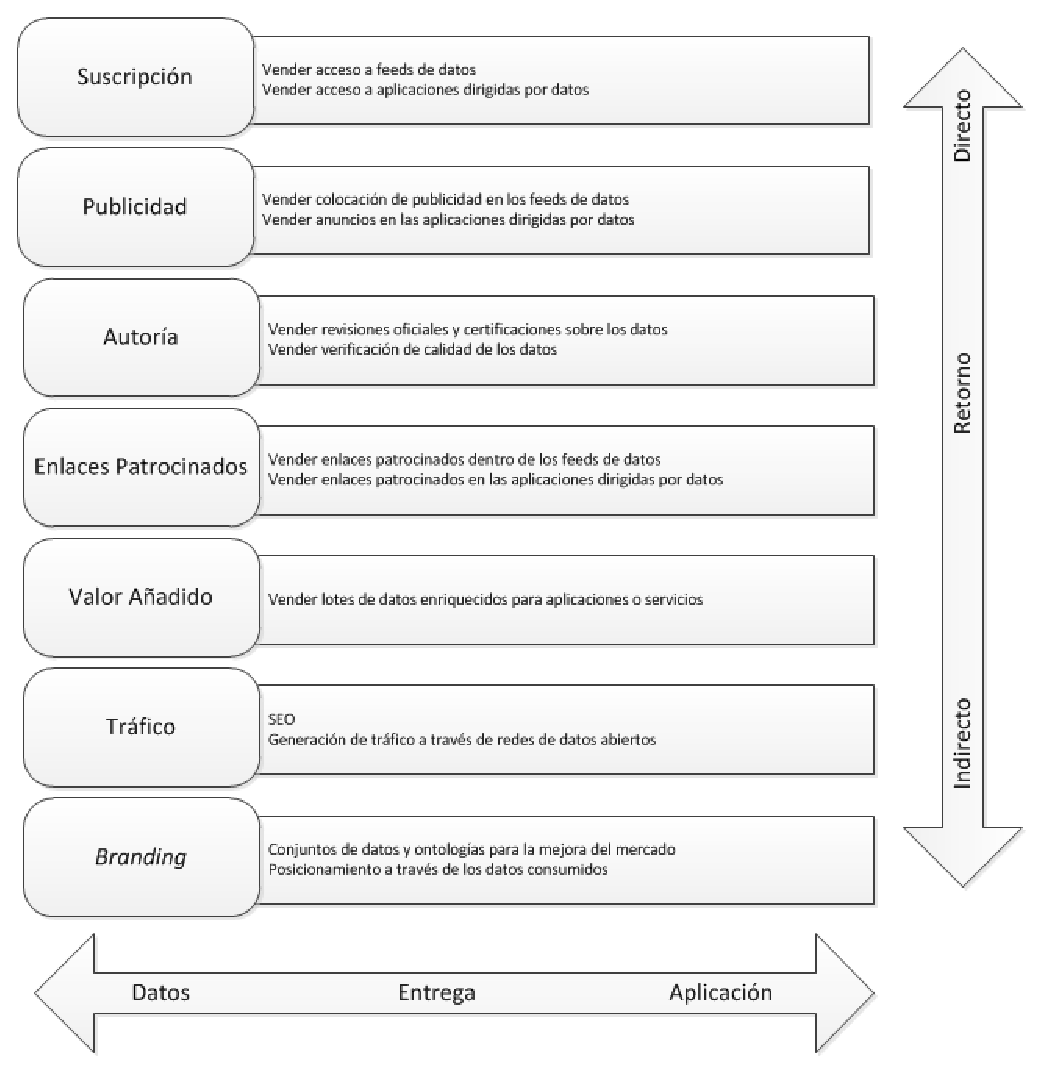
\includegraphics[width=12cm]{images/phd/data-business-models}
\caption{Modelos de negocio para datos.}
\label{fig:data-business-model}
\end{figure}


En definitiva, la conjunción de los principios de \linkeddata y \opendata ha conllevado una corriente de actuación
en las Administraciones Públicas con amplios beneficios tanto para los ciudadanos como para las empresas. La experiencia inicial es altamente
enriquecedora para las partes implicadas y su tendencia es seguir creciendo. No obstante, también se presentan varias cuestiones
abiertas que se habrán de ir resolviendo a la vez que la tecnología y la experiencia se incrementan.
\subsection{Principios de \linkeddata}\label{principos-linked-data}
En las secciones anteriores se han repasado las líneas que marcan la definición de \linkeddata, se pueden resumir
en una corriente que aúna la tecnología semántica más madura con la apertura de datos, en un infraestructura perfectamente
establecida como es la Web. Los principios de \linkeddata~\cite{Berners-Lee-2006} se reducen a los siguientes cuatro puntos:

\begin{itemize}
 \item \textit{Use \gls{URI}s as names for things}. La utilización de URIs como nombres para identificar y acceder a los recursos. Este principio busca el uso de URIs como camino para referenciar de forma única a todos
los recursos disponibles, no sólo documentos, así: contenidos digitales, vídeos, sensores~\cite{ontology-search,Jeung:2010:EMM:1850003.1850235}, 
  organizaciones~\cite{open-corporates}, personas~\cite{facebook-ld}, etc., con el objetivo de ampliar el contexto de un espacio virtual a uno real.
 \item \textit{When someone looks up a URI, provide useful information, using the standards (RDF*, SPARQL~\cite{Sparql})}. El acceso 
a los recursos a través de URIs debe estar basado en estándares como \gls{RDF} o \gls{SPARQL} proveyendo igualmente información
sobre el mismo.
\item \textit{Include links to other URIs. so that they can discover more things}. El enlazado de datos no sólo implica la publicación
masiva de los mismos, sino que se deben establecer enlaces entre ellos con el objetivo de proveer un entorno 
navegable~\cite{Berners-lee06tabulator:exploring,Pietriga06fresnel} y de consulta~\cite{Hartig09executingsparql}.
\item \textit{Use \gls{HTTP URI}s so that people can look up those names}. La utilización de URIs HTTP para reaprovechar la actual infraestructura
de la web y que el público potencial pueda acceder a los datos de la misma forma que se realiza actualmente con los documentos.
\end{itemize}

En general estos principios buscan una manera estándar de identificar, modelar, acceder y consumir recursos para que la creación
de aplicaciones y servicios sea lo más sencilla y ágil posible. Por lo tanto, 
para atender a estos principios se deben facilitar una serie de mecanismos que permitan:
\begin{itemize}
 \item Nombrar a todas las cosas, recursos, etc., mediante URIs.
 \item Referenciar y acceder a los contenidos mediante URIs. Uso de \textit{hash}, \textit{slash} URIs o código $303$ de \gls{HTTP}. 
 \item Proveer información útil sobre los recursos de forma estándar mediante RDF. Uso de literales o de enlaces a otras
descripciones RDF. Negociación de contenido.
 \item Incluir enlaces a otros datos. Podemos establecer tres tipos de enlaces principales: relación, identidad y 
vocabulario. Cada uno permite establecer relaciones, alinear unos recursos con otros y definir las descripciones
respectivamente.
\end{itemize}

Los beneficios de la utilización de estos mecanismos que sustentan a los cuatro principios citados proporcionan las siguientes ventajas:
\begin{itemize}
 \item Escala global. El uso de \gls{RDF} permite unificar la información de los recursos, modelo, formato y acceso a los datos.
 \item Enlace entre recursos. RDF da soporte a la reutilización intrínseca de recursos ya definidos dando cabida
a la unión de datos de diferentes fuentes.
  \item Expresividad. La información en RDF se puede representar combinando distintos vocabularios.
 \item Estructuración. Utilizando un modelo definido en RDF(S) u \gls{OWL} se da soporte al modelo de los datos
mediante mecanismos estándar, compartidos y reutilizables.
\end{itemize}

Además de estas ventajas, existen ciertas características que deberían evitarse, tales como los mecanismos
de reificación de RDF, las colecciones o el uso de nodos en blanco con el objetivo de facilitar la consulta
mediante el lenguaje SPARQL. En cuanto a los formatos en los que se pueden presentar los datos enlazados en RDF se encuentra:
\gls{RDFa}~\cite{rdfa-primer}, \gls{RDF/XML}~\cite{rdf-syntax}, \gls{Turtle}~\cite{turtle-syntax}, \gls{N3}~\cite{n3-syntax}, \gls{RDF}/\gls{JSON}~\cite{rdf-binario} o RDF binario~\cite{rdf-json}.


En definitiva, se trata de proveer un entorno estándar y global de datos en el cual se utilice un modelo
de datos estandarizado y único (RDF), con capacidad para enlazar a otros datos y que todos ellos se autodescriban
en el sentido de facilitar a sus descripciones beneficiando el descubrimiento, acceso e integración de datos.

\subsection{Construyendo una nueva \wod}
Este nuevo entorno de publicación de datos ha implicado que numerosas personas y organizaciones
se hayan inclinado por la aplicación de los principios de los datos enlazados en la apertura de sus datos. Como resultado
se puede establecer que el despegue de la \wod es ya un hecho, creando un grafo global de billones
de tripletas RDF de diferentes tipos y fuentes enlazadas~\cite{HoganUHCPD:2012:237} entre sí. En general, esta eclosión se debe
a varias razones: genericidad, estandarización, dominio público, capacidad de representación de la información, expresividad,
reutilización de tecnología estable, etc. Como origen de este enfoque se puede situar la iniciativa
del \lod~\cite{lod-group} (\gls{LOD}) del W3C en el año 2007, en el cual se sentaron las bases de la actual \wod, dando comienzo el desarrollo tecnológico así como la transformación de los primeros conjuntos de datos. Entre ellos
podemos destacar el esfuerzo de la DBPedia~\cite{dbpedia2009} o herramientas como \gls{Pubby}, D2RServer, etc. La evolución
de la \wod queda recogida en el diagrama de la nube de \datasets (\textit{LOD Cloud}~\cite{linked-data-cloud}) que en su última
versión recoge hasta 320 \datasets, ver Figura~\ref{fig:lod-cloud}, y continua en aumento si se consulta \textit{The Data Hub}~\cite{the-data-hub}. A modo informativo a fecha de septiembre
de 2010 en el diagrama anteriormente citado estaban disponibles unos 203 \textit{datasets} (en diciembre
de 2011 llegan hasta 326), más de 25 billones de tripletas \gls{RDF} y unos 395 millones de enlaces entre los diferentes datos.

\begin{figure}[!htb]
\centering
	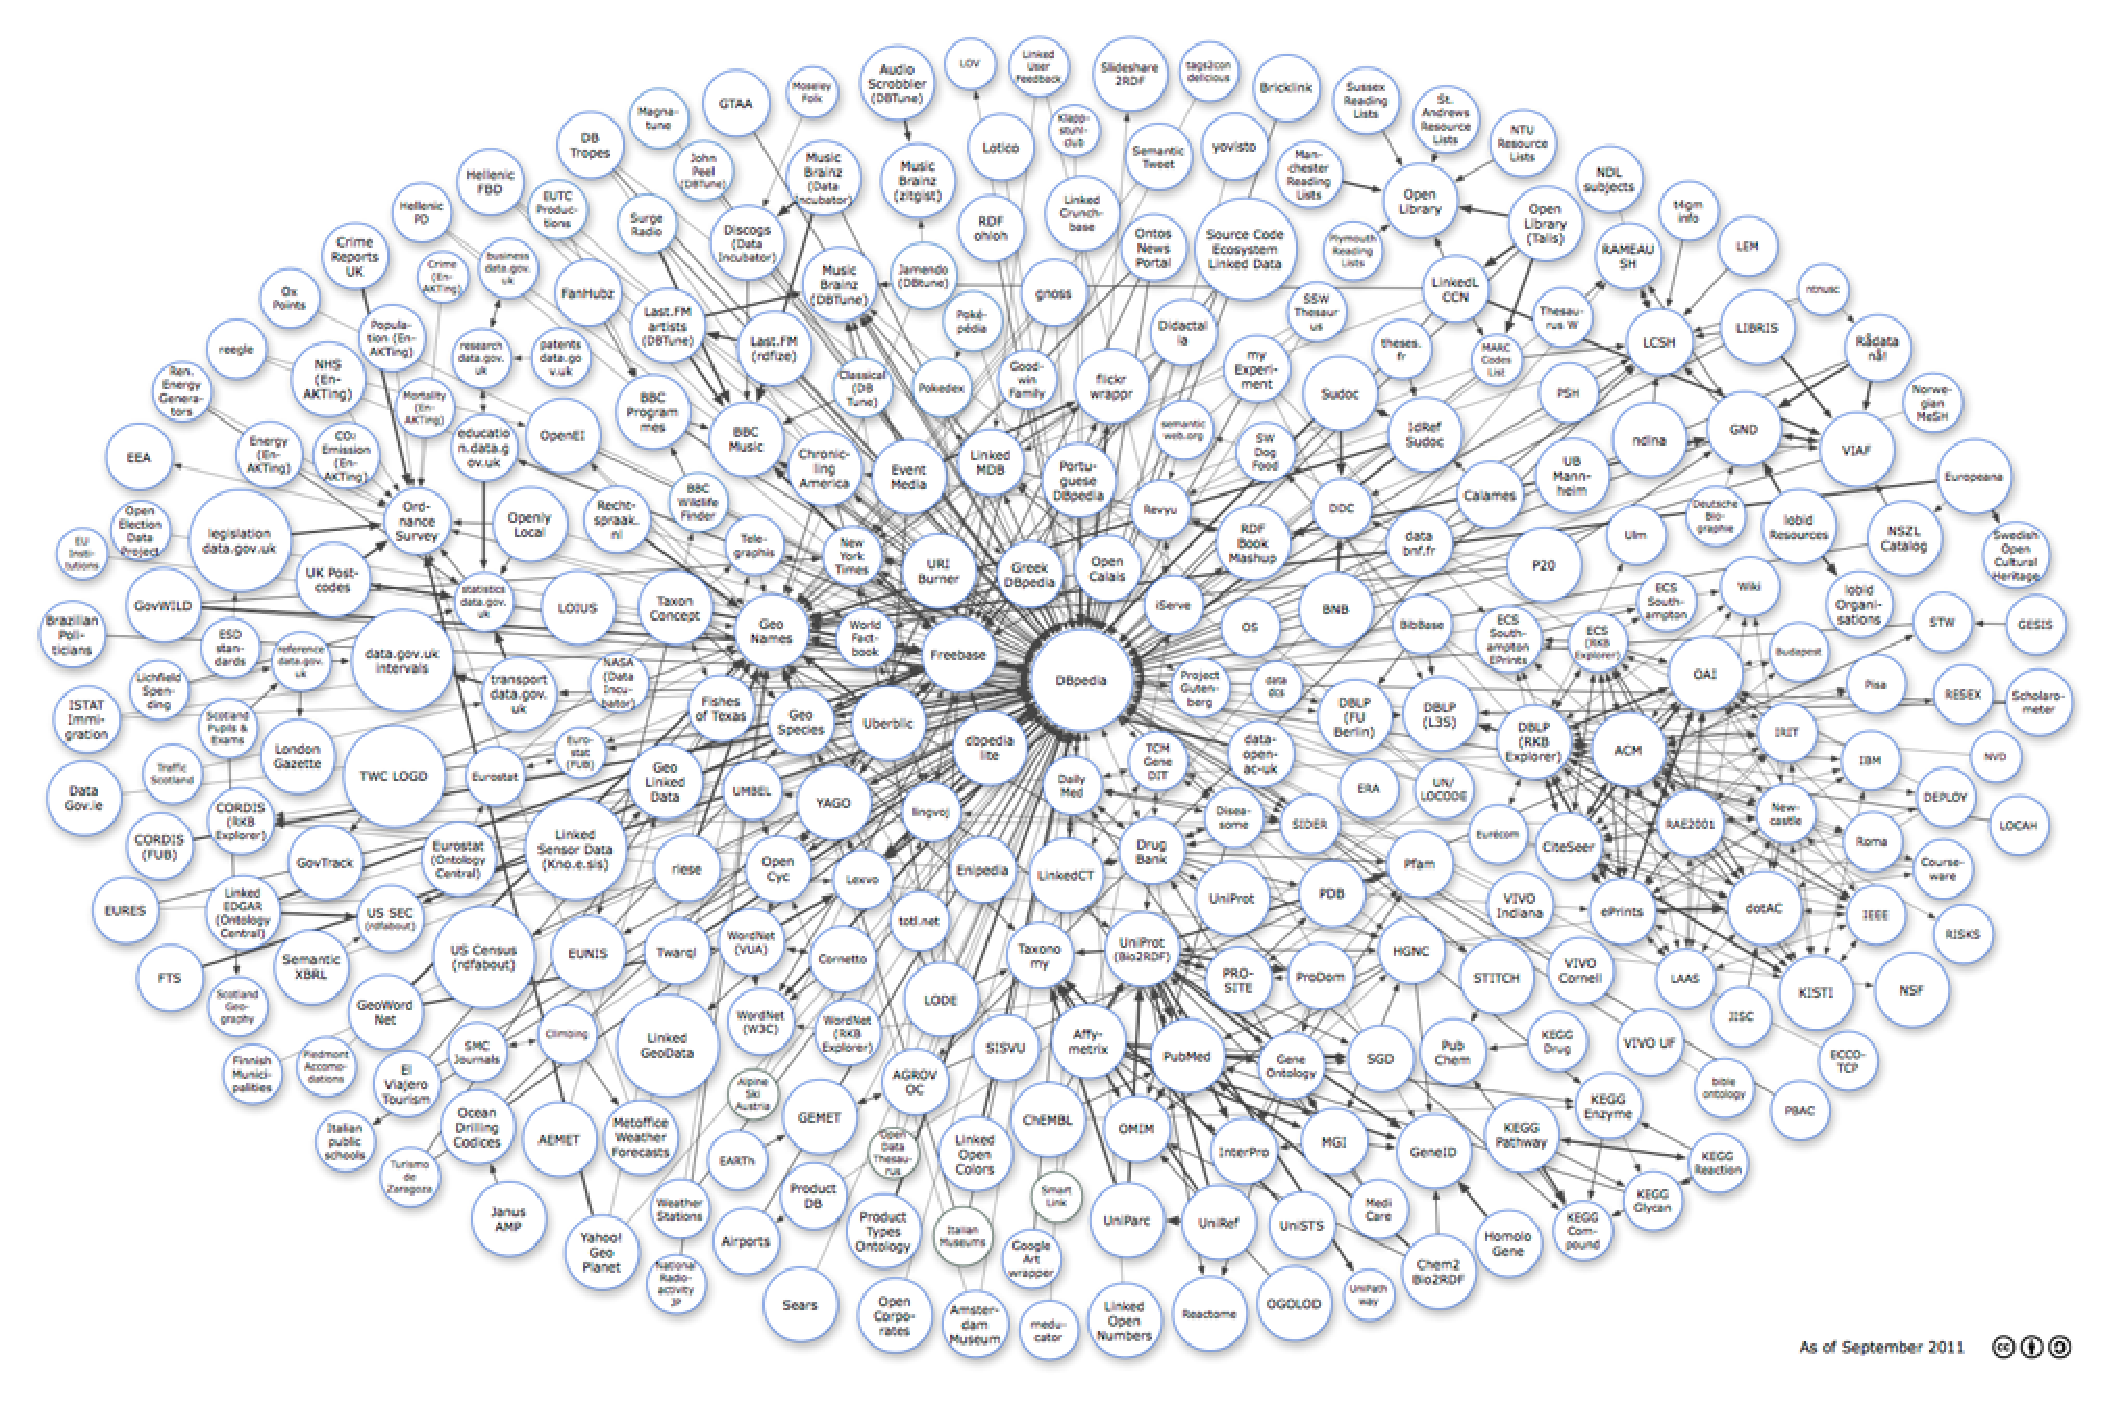
\includegraphics[width=10cm]{images/phd/lod-datasets_2011-09-19_1000px}
\caption{\textit{Linking Open Data cloud diagram, by Richard Cyganiak and Anja Jentzsch}.}
\label{fig:lod-cloud}
\end{figure}

Por otra parte, la información que se puede encontrar en la nueva \wod es tan variada como en la actual
web de documentos, a continuación algunos de los ejemplos de los datos que podemos encontrar, así:

\begin{itemize}
 \item Genéricos o de carácter transversal, candidatos a ser reutilizados por cualquier conjunto de datos: DBPedia~\cite{Bizer:2009:D-C:1640541.1640848}, 
Freebase~\cite{freebase}, etc.
 \item Geográficos: Geonames~\cite{geonames}, OpenStreetMap~\cite{open-street-maps} o GeoLinkedData~\cite{SLHA11}.
 \item ``Government Data'': Data Gov UK, Datos.es, etc.
 \item Educación, Multimedia, Bibliográficos, Científicos, Médicos, ``Social Media'', etc., que se pueden encontrar clasificados
en la versión del diagrama de la nube de \lod bajo diferentes colores.
\end{itemize}

A la hora de unirse a la \wod hay que tener en cuenta varias consideraciones, además de proveer
datos enlazados se deben tener en cuenta unos principios relativos al diseño:

\begin{description}
 \item [Diseño de las \gls{URI}s.] El objetivo es que las URIs referencien a objetos reales y que se puedan obtener
descripciones a través de los protocolos propios de Internet, requisito alineado directamente con el segundo principio de datos
enlazados y en este sentido hay que tener en cuenta varios aspectos: 
\begin{itemize}
 \item Uso de ``minting \gls{HTTP URI}s'': son URIs que están bajo el control de áquel que publica datos, es decir, utiliza
las URIs de su dominio para los datos y documentos.
\item ``Cool URIs''~\cite{Sauermann+2007a,bernerslee1998uri}: las URIs deben permanecer en el tiempo, en todo caso los usuarios las pueden cambiar, pero los identificadores
deberían permanecer inalterados. De la misma forma, se debe proveer un mecanismo para que a través de una misma URI se pueda
acceder a distinto contenido mediante negociación de contenido, extensiones, etc. 
\item ``Meaningful URIs'' vs ``ID based URIs''~\cite{uris-uk}: al igual que en el punto anterior se está ante la tesitura
de diseñar identificadores que se puedan recordar y con significado respecto a su contenido o bien utilizar
identificadores autogenerados. En cualquier caso, la decisión dependerá de la información a identificar, pero 
hay que tener presente este factor como clave en el diseño de la identificación de datos.
\end{itemize}
\item [Descripción de recursos con \gls{RDF}.] En este sentido se han establecido una serie de buenas prácticas y patrones
para describir los datos de los recursos susceptibles de publicación, ver Sección~\ref{metodologias}. Es importante seguir estas guías con el objeto de facilitar
su consulta a través de lenguajes como \gls{SPARQL}.
\item [Metainformación sobre los datos publicados.] No se trata sólo de publicar datos, ni de la apertura de las bases de datos
a la web, sino también de suministrar información sobre qué, cómo y dónde se puede acceder a estos datos. Para ello,
se debe atender a los siguientes criterios:
\begin{itemize}
 \item Usar vocabularios para describir el \dataset como \gls{voID}~\cite{void} o ``Semantic Sitemaps''\cite{Cyganiak08semanticsitemaps}.
 \item Añadir información sobre la procedencia~\cite{DBLP:conf/ipaw/HartigZ10,w3c-prov} de los datos (\provenance).
 \item Añadir información sobre la licencia~\cite{ld-licencias} de uso de los datos y los derechos de autoría, copia, distribución y modificación.
 \item Añadir información sobre la evolución temporal~\cite{ld-memento}, se puede conseguir mediante diferentes técnicas, incluyendo
la información en las URIs, en las descripciones RDF o mediante negociación de contenido.
\end{itemize}

\item [Seleccionar vocabularios a utilizar.] Existe un gran número de vocabularios~\cite{dcat-w3c} diseñados para describir
diversos tipos de información. La tendencia es reutilizar los vocabularios existentes~\cite{lod-stats} en la medida de lo posible, 
evitando remodelar información ya descrita. Aunque existen catálogos de vocabularios, finalmente es la experiencia
y la consulta de otros \datasets la principal vía de información para seleccionar los vocabularios a reutilizar.
En general se atenderá a los siguientes factores: uso actual, mantenimiento, cobertura y expresividad.

\item [Enlazar con otros ``\datasets''.] Al igual que en el punto anterior no existe una forma estándar
de realizar este proceso, puede ser manual o automático, pero si que es necesario fijar la atención en la semántica del enlace y seleccionar aquellos recursos que sean
de mayor uso para asegurar de nuevo la coherencia de los datos y su difusión.

\item [Publicar los datos.] Una vez determinados los datos a publicar, los cuales se han transformado y enlazado (si resultara oportuno), es
necesario proceder a su publicación de forma estandarizada mediante la aplicación de ciertos patrones definidos y teniendo en cuenta
si los datos son o no dinámicos, la criticidad, el esfuerzo de duplicar bases de datos, los formatos que van a ser soportados,
la exposición mediante servicios de consulta, el uso de un API, etc.
\item [Consumir datos publicados.] Este proceso conlleva la explotación de los datos disponibles tanto para generar
nuevos servicios de negocio o simplemente para consultar la información que se haya publicada y que se 
puede enriquecer con el universo de los demás \textit{datasets} publicados.
\item [Difundir los datos publicados.] Aunque no se trata de una acción o requisito funcional, el éxito de un conjunto
de datos publicados dependerá en buena medida, además de su calidad~\cite{ld-quality} y facilidad de acceso, de la difusión que se realice
sobre su uso y capacidad. Para ello, existen diversos catálogos~\cite{TummarelloDO07} y herramientas de indexado, por ejemplo
\textit{thedatahub.org}, \textit{prefix.cc}, etc., en los cuales se pueden incluir los datos publicados para que así, terceros 
los puedan consumir. La información de difusión deberá incluir aspectos relativos sobre cómo acceder a los datos, qué datos están publicados, el tipo de licencia, etc., para asegurar la confianza necesaria en los usuarios finales.

\end{description}

Como se ha reseñado en los puntos anteriores, pese a que existen patrones, recetas y métodos de producción, publicación y consumo de datos
es decisión del responsable la selección de los mismos. Si bien la flexibilidad de actuación queda patente y beneficia
la publicación masiva de datos, lleva consigo una desventaja, que reside en la posibilidad de errar en ciertos puntos provocando
una baja calidad en los datos. Para ello, tal y como se expone en la siguiente sección existen diversos esfuerzos para poner en común
estas guías bajo una metodología, especificando las actividades, participantes, herramientas y productos de entrada y salida
en cada una de las partes del proceso. En el objeto de este estudio, esta situación es de especial relevancia para poder evaluar las ventajas
de uso de datos enlazados, en contraposición con la actual situación de manejo de datos en el campo de la contratación pública
electrónica.

\subsection{Metodologías y Buenas Prácticas}\label{metodologias}
En las anteriores secciones se han presentando las diferentes iniciativas en torno a datos enlazados en un contexto
general, pero teniendo presentes las necesidades de la administración pública electrónica. Han quedado patentes las necesidades,
ventajas y algunas desventajas del uso de esta iniciativa para los procesos de producción, publicación y consumo de datos. Si 
bien existen muchas guías y principios de diseño que se pueden extraer a través de la literatura, es conveniente repasar
los enfoques que se están desarrollando para realizar una guía sobre cómo se deben aplicar los conceptos de  \linkeddata, \opendata, \ogd, \lod, etc., 
para ello existen diferentes guías e incluso plataformas que aglutinan una serie de características de interés que a continuación se listan, 
repasando las más destacadas.

\begin{itemize}
 \item \textit{Linked Data Design Considerations} del libro \textit{Linked Data: Evolving the Web into a Global Data Space}~\cite{Heath_Bizer_2011}.
 \item \textit{Linked Data Patterns}~\cite{linked-data-patterns}.
 \item \textit{Best Practices}~\cite{best-gld,Berr08} del grupo de trabajo del \gls{W3C} \textit{Government Linked Data First \gls{F2F} June 29-30, 2011}~\cite{gld-group}.
 \item \textit{Linked Data Cookbook}~\cite{linked-data-cookbook} del grupo de trabajo del W3C \textit{Government Linked Data Working Group}~\cite{gld-group}.
 \item \textit{Government Linked Data-Life Cycle}~\cite{gld-lifecycle} del grupo de trabajo del W3C \textit{Government Linked Data Working Group}.
 \item \textit{Publishing Open Government Data}~\cite{publishing-ogd} borrador de trabajo del W3C.
 \item \textit{LOD2 Stack}~\cite{lod2-stack} del proyecto europeo \textit{LOD2}~\cite{lod2-project}.
 \item \textit{Toward a Basic Profile for Linked Data}~\cite{basic-profile-w3c,basic-profile-ibm} de IBM.
 \item Metodología~\cite{DBLP:conf/i-semantics/Cifuentes-SilvaSG11,methodologyCaepia2011} propuesta por la Universidad de Oviedo en el ámbito de la Biblioteca del Congreso de Chile.
 \item \textit{Talis Platform}~\cite{talis}.  
 \item \textit{Linked Open Data: The Essentials}~\cite{Bauer2012}.
\item Documentación específica de cada país e incluso región para el despliegue de \opendata.
\end{itemize}

El objetivo de estas guías es definir unas directrices sobre cómo publicar los datos para obtener una \wod de calidad. Además y en 
esta misma línea se están organizando continuamente conferencias, talleres, etc., específicos dentro de los grandes eventos científicos
para divulgar las actividades relacionadas con \linkeddata, como por ejemplo \textit{Consuming Linking Open Data}~\cite{cold} (\gls{COLD}), 
\textit{Linked Data On the Web}~\cite{ldow} (\gls{LDOW}), \textit{Social Data On the Web}~\cite{sdow} (\gls{SDOW}) o \textit{Linked Enterprise Data Patterns}~\cite{linked-enterprise-data-patterns} que sirven 
como concentrador de las actividades que se están realizando en este ámbito y que abordan los principales problemas 
que aparecen en este entorno emergente.

\subsubsection{\textit{Linked Data Design Considerations}}\label{linked-data-design-issues}
En el libro~\cite{Heath_Bizer_2011} realizado por Chris Bizer (investigador en la Freie Universitat de Berlin, Alemania y creador de la DBPedia) y 
por Tom Heath (uno de los investigadores principales de la plataforma Talis~\cite{talis}) se ponen de manifiesto una serie de consideraciones, ver Tabla~\ref{table:linkeddata-design-book}
de diseño a tener en cuenta cuando se pretende desplegar una plataforma de datos enlazados. 


\begin{longtable}[c]{|l|p{6.5cm}|p{7.5cm}|} 

\hline

  \textbf{ID} & \textbf{Directriz} &  \textbf{Descripción} \\\hline

\endhead
   1& \multicolumn{2}{|c|}{\textbf{\textit{Using URIs as Names for Things}}}\\ \hline
   1.1 &  \textit{Minting \gls{HTTP URI}s} & Las URIs deben permitir acceder a los recursos que nombran. Uso del esquema HTTP. \\ \hline
   1.2 &  \textit{Use of Cool URIs} &  Las URIs deben seguir unos criterios de diseño que permitan y animen a terceros su uso.\\ \hline
   1.3 &  \textit{Keep out of namespaces you do not control} &  Las URIs de los recursos deben pertenecer a un dominio sobre el que se tenga control.\\ \hline
   1.4 &  \textit{Abstract away from implementation details} & Las URIs no incluyen detalles de implementación como el formato del recurso. \\ \hline
   1.5 &  \textit{Use Natural Keys within URIs} &  Para asegurar que las URIs son únicas se utiliza una clave primaria o ID para identificar recursos.\\ \hline
   1.6 &  \textit{Hash URIs} &  La concatenación de identificadores en el URI se realiza utilizando \# como separador final del recurso.\\ \hline
   1.7 &  \textit{Slash URIs} &  Igual que en el caso anterior pero utilizando $/$. \\ \hline
   2&\multicolumn{2}{|c|}{\textbf{\textit{Describing Things with RDF}}}\\ \hline
   2.1 &  \textit{\gls{RDF} resources} & Cuando se accede a un recurso a través de un \gls{URI} se debe proveer información útil. \\ \hline
   2.2 &  \textit{Literal Triples and Outgoing Links} & El sujeto de la información en RDF es siempre el URI del recurso que se está describiendo. \\ \hline
   2.3 &  \textit{Incoming Links} & Proveer enlaces a otros recursos para hacer los datos navegables. \\ \hline
   2.4 &  \textit{Triples that Describe Related Resources} & Describir parcialmente los recursos que son enlazados desde el actual. \\ \hline
   2.5 &  \textit{Triples that Describe the Description} & Añadir metainformación sobre los propios recursos como licencia. \\ \hline
\newpage
  3&\multicolumn{2}{|c|}{\textbf{\textit{Publishing Data about Data}}}\\ \hline
   3.1 &  \textit{Describing a Data Set} & Añadir metainformación sobre el conjunto de datos que se está publicando. \\ \hline
   3.2 &  \textit{Use of Semantic Sitemaps} & Utilizar la extensión de \textit{Sitemap} para describir los datos proveyendo capacidades nuevas para los buscadores. \\ \hline
   3.3 &  \textit{Use of voiD Descriptions} & Utilizar el vocabulario voiD (\textit{the Vocabulary of Interlinked Datasets}) para la metainformación de los datos. Es considerado el estándar de facto. \\ \hline
   3.4 &  \textit{Provenance Metadata} & Añadir información sobre la procedencia de los datos. Capacidades de monitorización y evolución en el tiempo. \\ \hline
   3.5 &  \textit{Licenses, Waivers and Norms for Data} & Incluir información sobre el uso posible de los datos a través de una licencia. \\ \hline
   3.6 &  \textit{Non-copyrightable Material} & $\approxeq$ \\ \hline
   4&\multicolumn{2}{|c|}{\textbf{\textit{Choosing and Using Vocabularies to Describe Data}}}\\ \hline
   4.1 &  \textit{\gls{SKOS}, RDFS and \gls{OWL}} &  Modelar la información de los datos de acuerdo a un vocabulario estándar. Proveer un modelo formal para los datos.\\ \hline
   4.2 &  \textit{Annotations in RDFS} &  Usar las anotaciones \texttt{rdfs:label} y \texttt{rdfs:comment} en las descripciones de RDF.\\ \hline
   4.3 &  \textit{Relating Classes and Properties} &  Relacionar los recursos en RDF mediante propiedades de RDFS, SKOS, etc.: \texttt{rdfs:subClassOf}, \texttt{skos:related}, etc.  \\ \hline
   4.4 &  \textit{Reusing Existing Terms} & Reutilizar las definiciones ya concebidas en los vocabularios existentes de los distintos dominios como: Dublin Core, FOAF, etc. \\ \hline
   4.5 &  \textit{Selecting Vocabularies} & Seleccionar los vocabularios a reutilizar teniendo en cuenta: \textit{Usage and uptake}, \textit{Maintenance and governance}, \textit{Coverage} y \textit{Expressivity}.\\ \hline
   4.6 &  \textit{Defining Terms} &  Si los vocabularios existentes no cubren las necesidades de nuestros datos, definir nuevos términos.\\ \hline
   5&\multicolumn{2}{|c|}{\textbf{\textit{Making Links with RDF}}}\\ \hline
   5.1 &  \textit{Publishing Incoming and Outgoing Links} &  Publicar un volcado de los datos en RDF.\\ \hline
   5.2 &  \textit{Making Links with External Data Sources} &  Reutilizar y enriquecer las descripciones en RDF con otras ya existentes asegurando que existen.\\ \hline
   5.3 &  \textit{Choosing External Linking Targets} & Los enlaces a datos externos deben cumplir que sean referenciables mediante un URI y deberían ser reutilizados por otros.\\ \hline
   5.4 &  \textit{Choosing Predicates for Linking} & Similar al punto $22$.\\ \hline
   5.5 &  \textit{Setting RDF Links Manually} & Incluir enlaces en las descripciones en RDF mediante edición manual (si de forma automática no es fiable).\\ \hline
   5.6 &  \textit{Auto-generating RDF Links} & Incluir enlaces las descripciones en RDF de forma automática. Uso de herramientas de reconciliación de entidades: SILK, LIMES, etc.\\ \hline
   5.7 &  \textit{Key-based Approaches} & Los enlaces se realizan mediante búsqueda de recursos con palabras claves.\\ \hline
   5.8 &  \textit{Similarity-based Approaches} & Los enlaces se realizan mediante búsqueda de recursos de acuerdo a una estructura.\\ \hline
  6&\multicolumn{2}{|c|}{\textbf{\textit{Recipes for Publishing Linked Data}}}\\ \hline
   6.1 &  \textit{Linked Data Publishing Patterns} & Establecer el modelo para ofrecer los datos.\\ \hline
   6.2 &  \textit{From Queryable Structured Data to Linked Data} & Exportar una base de datos relacional mediante un mapeador a RDF.\\ \hline
   6.3 &  \textit{From Static Structured Data to Linked Data} & Transformar datos estáticos a RDF. Por ejemplo: CSV, MSExcel, etc.\\ \hline
   6.4 &  \textit{From Text Documents to Linked Data} & Extraer los datos RDF de documentos de texto.\\ \hline
   6.5 &  \textit{Data Volume: How much data needs to be served?} & Dependiendo de la cantidad de datos definir qué datos y cantidad se pueden exportar.\\ \hline
   6.6 &  \textit{Data Dynamism: How often does the data change?} & Dependiendo de los cambios en los datos definir qué patrón se adapta mejor a la exportación de los datos.\\ \hline
   6.7 &  \textit{Serving Linked Data as Static RDF/XML Files} & Publicar los ficheros en RDF en un servidor web. Forma más sencilla.\\ \hline
   6.8 &  \textit{Hosting and Naming Static RDF Files} & Utilizar una convención de nombrado y negociación de contenido para los ficheros en RDF. Reglas de reescritura en servidor web.\\ \hline
   6.9 &  \textit{Server-Side Configuration: \gls{MIME} Types} & Servir el contenido apropiado de acuerdo a los tipos MIME.\\ \hline
   6.10 &  \textit{Making RDF Discoverable from \gls{HTML}} & Permitir que desde HTML se puedan reutilizar las descripciones en RDF.\\ \hline
   6.11 &  \textit{Serving Linked Data as RDF Embedded in HTML Files} & Enriquecer HTML con las descripciones en RDF. Por ejemplo con RDFa.\\ \hline
   6.12 &  \textit{Serving RDF and HTML with Custom Server-Side Scripts} & Generación bajo demanda de RDF en el servidor.\\ \hline
   6.13 &  \textit{Serving Linked Data from Relational Databases} & Generación bajo demanda de RDF en el servidor \textit{mapeando} a una base de datos.\\ \hline
   6.14 &  \textit{Serving Linked Data from RDF Triple Stores} & Utilizar las capacidades de un triple-store para ofrecer RDF.\\ \hline
   6.15 &  \textit{Serving Linked Data by Wrapping Existing Application or Web \gls{API}s} & Exportar los datos de las aplicaciones web existentes como RDF.\\ \hline
   6.16 &  \textit{Testing and Debugging Linked Data} & Utilizar herramientas para verificar que se cumple con los principios de \linkeddata y de la publicación de datos.\\ \hline
   7&\multicolumn{2}{|c|}{\textbf{\textit{Architecture of Linked Data Applications}}}\\ \hline
   7.1 &  \textit{The Crawling Pattern} & Se navega por los recursos RDF con el objeto de extraer los datos para proveer servicios y datos a una capa superior.\\ \hline
   7.2 &  \textit{The On-The-Fly Dereferencing Pattern} & El patrón de los navegadores de \linkeddata que extraen la información de los recursos en el momento en el que se necesita.\\ \hline
   7.3 &  \textit{The Query Federation Pattern} & Se crean consultas complejas ejecutadas sobre varias fuentes de datos que se presentan al usuario dentro de una aplicación.\\ \hline
 
\hline
\caption{Consideraciones de Diseño \linkeddata}\label{table:linkeddata-design-book}\\    
\end{longtable}

Como se puede comprobar, en esta lista residen una serie de consideraciones a valorar en relación con la producción, publicación y consumo de datos
enlazados. La implementación o el uso que se realice de cada uno de estos puntos depende de la estrategia seguida por la persona o institución
implicada en el proceso de ofrecer sus datos bajo la iniciativa \linkeddata. Finalmente y tras aplicar estos principios se puede utilizar
el siguiente \textit{checklist}, es similar al utilizado para añadir un conjunto de datos a la iniciativa \gls{LOD} Cloud,
 para verificar, ver Tabla~\ref{table:linkeddata-check-list}, si se han aplicado de forma correcta los principios de diseño propuestos por los autores y en consecuencia de \linkeddata.


\begin{longtable}[c]{|l|p{6.5cm}|p{7.5cm}|} 

\hline

  \textbf{ID} & \textbf{Punto a cumplir} &  \textbf{Descripción} \\\hline

\endhead
   1 &  \textit{Does your data set links to other data sets?} & Existen enlaces externos desde las descripciones en RDF a otros externos que conformen un grafo global .\\ \hline
   2 &  \textit{Do you provide provenance metadata?} &  Los datos disponen de información sobre su procedencia.\\ \hline
   3 &  \textit{Do you provide licensing metadata?} &  Se establecen las restricciones necesarias sobre el uso de los datos.\\ \hline
   4 &  \textit{Do you use terms from widely deployed vocabularies?} & Las descripciones en \gls{RDF} se basan en reutilizar clases y propiedades ya existentes y aplicadas ampliamente. \\ \hline
   5 &  \textit{Are the URIs of proprietary vocabulary terms dereferenceable?} & Las clases y propiedades definidas particularmente son referenciables. \\ \hline
   6 &  \textit{Do you map proprietary vocabulary terms to other vocabularies?} &  Las clases y propiedades definidas se basan y relacionan con otras ya existentes y aplicadas ampliamente.\\ \hline
   7 &  \textit{Do you provide data set-level metadata?} &  Se ofrece metainformación sobre el conjunto de datos en general\\ \hline
   8 &  \textit{Do you refer to additional access methods?} &  Además del uso de \gls{URI}s para referenciar los datos se proveen otros servicios como un \textit{endpoint} de SPARQL.\\ \hline

\hline
\caption{\textit{Checklist} \linkeddata}\label{table:linkeddata-check-list}\\    
\end{longtable}

% \begin{figure}[!htb]
% \centering
% 	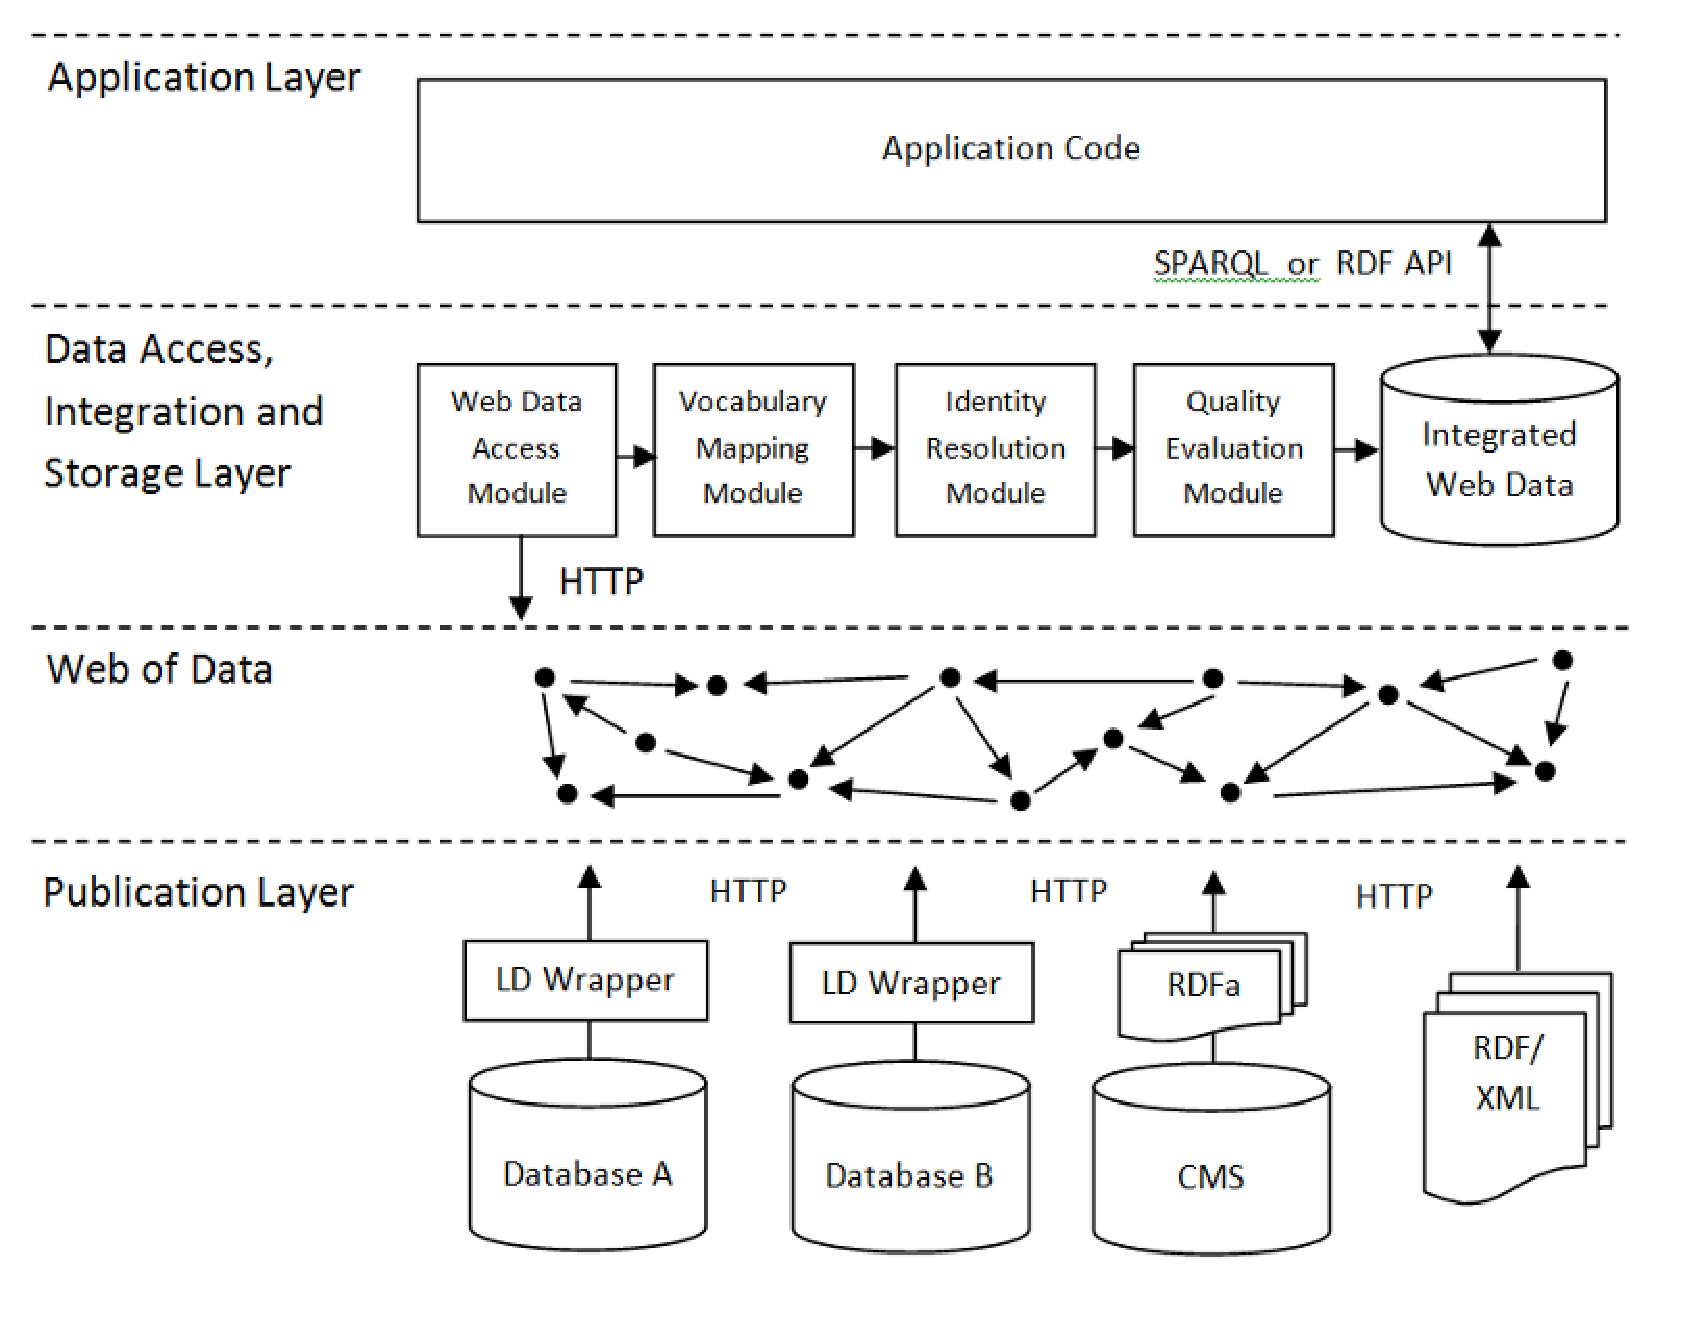
\includegraphics[width=10cm]{images/phd/Consumingarchitecture1_small}
% \caption{\textit{Linked Data Publishing Options and Workflows} (extraída de \textit{Linked Data Design Considerations}).}
% \label{fig:patterns-production}
% \end{figure}

En conclusión, en este libro se ofrece una guía práctica y didáctica de los pasos a seguir para la aplicación
de la iniciativa de \linkeddata de forma correcta, asegurando las ventajas presentes en los datos enlazados, minimizando las desventajas
y proveyendo un entorno para la generación de servicios de alto valor y calidad. 
Se observa que tanto las directrices de la Tabla~\ref{table:linkeddata-design-book}, como
los puntos a cumplir de la Tabla~\ref{table:linkeddata-check-list}, se pueden englobar en tres grandes procesos: producción,
publicación y consumo de \linkeddata. 
% Especialmente hay que destacar los enfoques para la producción de \linkeddata desde
% fuentes de datos ya existentes, ver Figura~\ref{fig:patterns-production} y Figura~\ref{fig:patterns-consum}.

% \begin{figure}[!htb]
% \centering
% 	\includegraphics[width=10cm]{images/phd/D2RServerArchitecture}
% \caption{Architectura de D2R Server.}
% \label{fig:patterns-consum}
% \end{figure}


\subsubsection{\textit{Linked Data Patterns}}\label{linked-data-patterns}
Con el objetivo de proveer una forma estándar de transformar los datos
siguiendo la iniciativa de \linkeddata y disponer de unos criterios y soluciones estándar
para modelar, publicar y consumir datos, se han publicado una serie de patrones~\cite{linked-data-patterns} que resuelven
los problemas más comunes que se pueden encontrar tales como el diseño de URIs, tipos de datos, etiquetado de 
recursos, etc. Al igual que en el caso anterior, en estos patrones se ofrecen una serie de guías para resolver problemas comunes
que surgen en el momento de producir, publicar y consumir datos enlazados. Suponen una información muy valiosa, ya que
permiten homogeneizar la creación de datos enlazados de tal forma que si una persona u organización asegura que ha 
seguido estos principios, se pueden construir aplicaciones que sepan qué tipo de datos se van encontrar y cómo, disminuyendo
así el coste de reutilización de datos provenientes de terceros y asegurar la calidad de los mismos.

%A continuación, ver Tabla~\ref{table:linkeddata-patterns}, se describen algunos de los propuestos por los autores:
% 
% 
% \begin{longtable}[c]{|l|p{7cm}|p{8cm}|} 
% 
% \hline
% 
%   \textbf{ID} & \textbf{Patrón} &  \textbf{Pregunta} \\\hline
% 
% \endhead
%    1& \multicolumn{2}{|c|}{\textbf{\textit{Identifier Patterns}}}\\ \hline
%   1.1 &  \textit{Hierarchical URIs} & \textit{How should URIs be assigned to a group of resources that form a natural hierarchy?}\\ \hline
%   1.2 &  \textit{Literal Keys} & \textit{How do we publish non-global identifiers in \gls{RDF}?} \\ \hline
%   1.3 &  \textit{Natural Keys} &  \textit{How can we create unique URIs from data that already has unique identifiers?} \\ \hline
%   1.4 &  \textit{Patterned URIs} & \textit{How can we create more hackable, human-readable URIs?} \\ \hline
%   1.5 &  \textit{Proxy URIs} & \textit{How do we deal with lack of standard identifiers for third-party resources?} \\ \hline
%   1.6 &  \textit{Shared Keys} & \textit{How do we simplify the inter-linking of datasets?} \\ \hline
%   1.7 &  \textit{URL Slug} &  \textit{How can we create \gls{URL}s from arbitrary text or keywords?} \\ \hline    
%     2& \multicolumn{2}{|c|}{\textbf{\textit{Modelling Patterns}}}\\ \hline
%   2.1 &  \textit{Custom Datatype} &  \textit{A data model contains structured values that don't correspond to one of the pre-existing \gls{XML Schema} datatypes.} \\ \hline    
%   2.2 &  \textit{Index Resources} &  \textit{How can ordered collections or indexes be published as RDF?}  \\ \hline    
%   2.3 &  \textit{Label Everything} & \textit{How can we ensure that every resource has a basic human-readable name?} \\ \hline     
%   2.4 &  \textit{Link Not Label} &  \textit{How do we model a dataset to maximise benefits of a graph based model?} \\ \hline    
%   2.5 &  \textit{Multi-Lingual Literal} & \textit{How can internationalized text be expressed in RDF? }\\ \hline    
%   2.6 &  \textit{N-Ary Relation} & \textit{How can a complex relation, involving several resources, be modelled as RDF? }\\ \hline    
%   2.7 &  \textit{Ordered List} &  \textit{How do we specify an ordering over a collection of resources?} \\ \hline     
%   2.8 &  \textit{Ordering Relation} & \textit{How can we specify an ordering relationship between two or more resources?} \\ \hline     
%   2.9 &  \textit{Preferred Label} &  \textit{How can a simple unambiguous label be provided for a resource? }\\ \hline    
%   2.10 &  \textit{Qualified Relation} &  \textit{How can we describe or qualify a relationship between two resources?} \\ \hline   
%   2.11 &  \textit{Reified Statement} &  \textit{How can we make statements about statements?} \\ \hline    
%   2.12 &  \textit{Topic Relation} &  \textit{How can a web page or document be associated with a resource?} \\ \hline      
%   2.13 &  \textit{Typed Literal} &  \textit{How can a datatype be associated with an RDF literal?} \\ \hline        
%     3& \multicolumn{2}{|c|}{\textbf{\textit{Publishing Patterns}}}\\ \hline
%   3.1 &  \textit{Annotation} &  \textit{How can data about third-party resources be published as part of a dataset?}  \\ \hline    
%   3.2 &  \textit{Autodiscovery} &   \textit{How can people find the underlying linked data for a given web page?}  \\ \hline    
%   3.3 &  \textit{Document Type} & \textit{How can some context be provided about a set of RDF triples published to the web?} \\ \hline     
%   3.4 &  \textit{Edit Trail} &  \textit{How can people be encouraged to improve or fix up open data?} \\ \hline    
%   3.5 &  \textit{Embedded Metadata} &  \textit{How do we add structured data to an existing document or file?} \\ \hline    
%   3.6 &  \textit{Equivalence Links} &  \textit{How do we indicate that different \gls{URI}s refer to the same resource or concept?} \\ \hline    
%   3.7 &  \textit{Link Base} &  \textit{How can outbound links from a dataset be managed separately from the core data?} \\ \hline     
%   3.8 &  \textit{Materialize Inferences} &  \textit{How can data be published for use by clients with limited reasoning capabilities?} \\ \hline     
%   3.9 &  \textit{Named Graphs} & \textit{How do we organize and annotate a set of RDF statements?} \\ \hline    
%   3.10 &  \textit{Primary Topic Autodiscovery} & \textit{How can people identify the principal subject of a given web page?}  \\ \hline    
%   3.11 &  \textit{Progressive Enrichment} &  How can the quality of data or a data model be improved over time? \\ \hline      
%   3.12 &  \textit{See Also} & \textit{How can RDF documents be linked together to allow crawlers and user agents to navigate between them?} \\ \hline    
%         4& \multicolumn{2}{|c|}{\textbf{\textit{Application Patterns}}}\\ \hline
%   4.1 &  \textit{Assertion Query} & \textit{How can a dataset be tested for known patterns?} \\ \hline    
%   4.2 &  \textit{Blackboard} &  \textit{How can the task of compiling or constructing a dataset be divided up into smaller tasks?}\\ \hline    
%   4.3 &  \textit{Bounded Description} & \textit{How can we generate a useful default description of a resource without having to enumerate all the properties or relations that are of interest?} \\ \hline     
%   4.4 &  \textit{Composite Descriptions} &  \textit{How do we declare the underlying dataset for a page involving custom subsets or views of the data?}\\ \hline    
%   4.5 &  \textit{Follow Your Nose} &  \textit{How do we find additional relevant data from the web?} \\ \hline    
%   4.6 &  \textit{Missing Isn't Broken} &  \textit{How do we handle the potentially messy or incomplete data we use from the web?} \\ \hline    
%   4.7 &  \textit{Parallel Loading} &  \textit{How can we reduce loading times for a web-accessible triple store?} \\ \hline     
%   4.8 &  \textit{Parallel Retrieval} & \textit{ How can we improve performance of an application dynamically retrieving Linked Data?} \\ \hline     
%   4.9 &  \textit{Resource Caching} &  \textit{How can an application that relies on loading data be more tolerant of network failures and/or reduce use of bandwidth} \\ \hline    
%   4.10 &  \textit{Schema Annotation} & \textit{How can application-specific processing rules be externalized?} \\ \hline    
%   4.11 &  \textit{Smushing} &  \textit{How do we merge data about resources that may not be consistently identified?} \\ \hline
%   4.12 &  \textit{Transformation Query} & \textit{How can we normalize or transform some RDF data so that it conforms to a preferred model?} \\ \hline        
%  
% \hline
% \caption{\textit{Linked Data Patterns}}\label{table:linkeddata-patterns}\\    
% \end{longtable}



\subsubsection{\textit{Best Practices} del W3C}
Se trata de una serie de documentos y buenas prácticas~\cite{best-gld} dentro del 
grupo de trabajo del \gls{W3C} \textit{Government Linked Data Working Group}~\cite{gld-group} cuya actividad se lanzó
 en el \textit{Face 2 Face} de junio de 2011 y que consta de los siguientes objetivos:

\begin{itemize}
 \item \textit{The overarching objective is to provide best practices and guidance to create of high quality, re-usable Linked Open Data (LOD)}.
 \item \textit{Description of the full life cycle of a Government Linked Data project, starting with identification of suitable data sets, procurement, modeling, vocabulary selection, through publication and ongoing maintenance.}
 \item \textit{Definition of known, proven steps to create and maintain government data sets using Linked Data principles.}
  \item \textit{Guidance in explaining the value proposition for LOD to stakeholders, managers and executives.}
  \item \textit{Assist the Working Group in later stages of the Standards Process, in order to solicit feedback, use cases, etc.}
\end{itemize}

Como grupo de trabajo su esfuerzo se centrará en cumplir los objetivos establecidos a través de la consecución de materiales como 
recomendaciones, notas, etc., en los siguientes ámbitos:
\begin{enumerate}
 \item  \textit{Procurement}.
 \item  \textit{Vocabulary Selection}.
 \item \textit{URI Construction}.
   \item \textit{Versioning} y \textit{Stability}.
   \item \textit{Legacy Data}.
   \item \textit{Cookbook}. 
\end{enumerate}

Evidentemente y teniendo en cuenta los participantes en esta actividad, está claro que los puntos de actuación
seleccionados son claramente estratégicos para la iniciativa de \linkeddata y es por ello que aunque
los resultados están en una etapa previa, es conveniente prestar suma atención a sus resultados con un doble objetivo, 
por una parte aplicarlos a futuros proyectos y por otra realimentar el esfuerzo realizado por sus participantes.

\subsubsection{\textit{Linked Data Cookbook} del W3C}\label{linked-data-cookbook}
Uno de los esfuerzos de la actividad comentada en la sección anterior, consiste
en la elaboración de un libro de buenas prácticas~\cite{linked-data-cookbook} en cuanto a la producción, publicación y consumo de 
datos enlazados. Para ello se recopilarán las prácticas más comunes
desde el punto de vista de la ingeniería que faciliten la adopción de \linkeddata en 
diferentes entornos, asegurando una calidad y previniendo que el uso de datos enlazados
no sea sinónimo de depuración.

Con carácter previo se han fijado una serie de pasos que se han de seguir para desplegar
una infraestructura de datos enlazados acompañada de una serie de prácticas que aseguren
la calidad y el proceso de adopción. Esta iniciativa es compatible con las buenas prácticas
señaladas en las Secciones~\ref{linked-data-design-issues} y~\ref{linked-data-patterns} y además
ofrece una buena guía de todos los puntos que hay que tener en cuenta: diseño de URIs, vocabularios
a reutilizar, herramientas, etc. Actualmente estas prácticas se están desarrollando y 
se dividen en $7$ pasos que se presentan en la Tabla~\ref{table:linkeddata-practices}.


\begin{longtable}[c]{|l|p{6.5cm}|p{7.5cm}|} 

\hline

  \textbf{ID} & \textbf{Práctica} & \textbf{Descripción} \\\hline

\endhead
  1 &  \textit{Model the Data} & \textit{Identify, Model, Name and Test.}\\ \hline
  2 &  \textit{Name things with \gls{URI}s} & \textit{Following a name convention of current guides.} \\ \hline
  3 &  \textit{Re-use vocabularies whenever possible} &   \textit{Any given Linked Data set may include terms from an existing and widely used vocabulary.} \\ \hline
  4 &  \textit{Publish human and machine readable descriptions} & \textit{Self-describing data suggests that ''information about the encodings used for each representation is provided explicitly within the representation``}.  \\ \hline
  5 &  \textit{Convert data to \gls{RDF}} & N/A \\ \hline
  6 &  \textit{Specify an appropriate license} & N/A \\ \hline
  7 &  \textit{Announce the new Linked Data Set(s) } &  N/A  \\ \hline    
 
\hline
\caption{\textit{The 7 Best Practices for Producing Linked Data.}}\label{table:linkeddata-practices}\\    
\end{longtable}


\subsubsection{\textit{Government Linked Data-Life Cycle}}\label{gld}
Siguiendo con las actividades que se desarrollan en este grupo de trabajo del W3C sobre datos enlazados
en el entorno de la administración pública electrónica, se han identificado los siguientes ciclos de vida~\cite{gld-lifecycle} propuestos
por diversos autores:

\begin{itemize}
 \item \textit{Bernadette Hyland}, ver Figura~\ref{fig:hyland}. 
 \item \textit{Michael Hausenblas}, ver Figura~\ref{fig:hausenblas}.
 \item \textit{Boris Villazón-Terrazas}, ver Figura~\ref{fig:boris}
 \item \textit{The DataLift Vision}, ver Figura~\ref{fig:datalift} 
 \end{itemize}


\begin{figure}[!htb]
\centering
	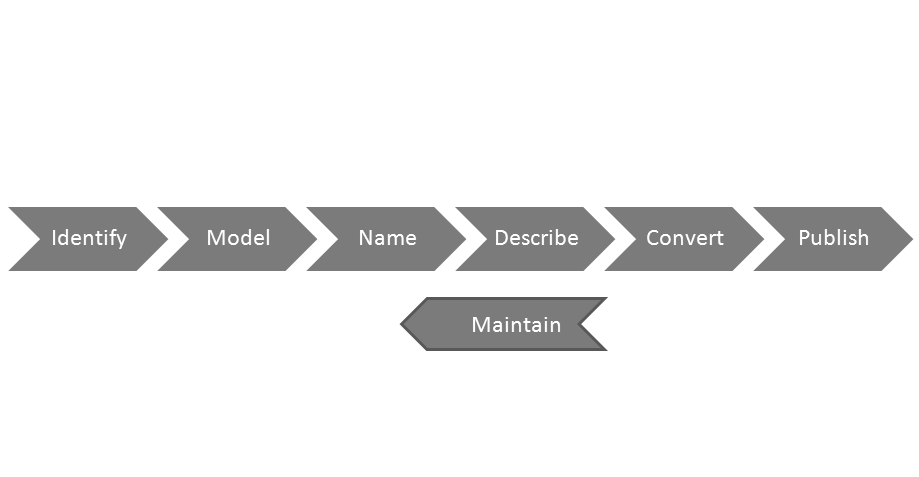
\includegraphics[width=14cm]{images/phd/Hyland}
\caption{\textit{Linked Data Lifecycle by B. Hyland}.}
\label{fig:hyland}
\end{figure}

\begin{figure}[!htb]
\centering
	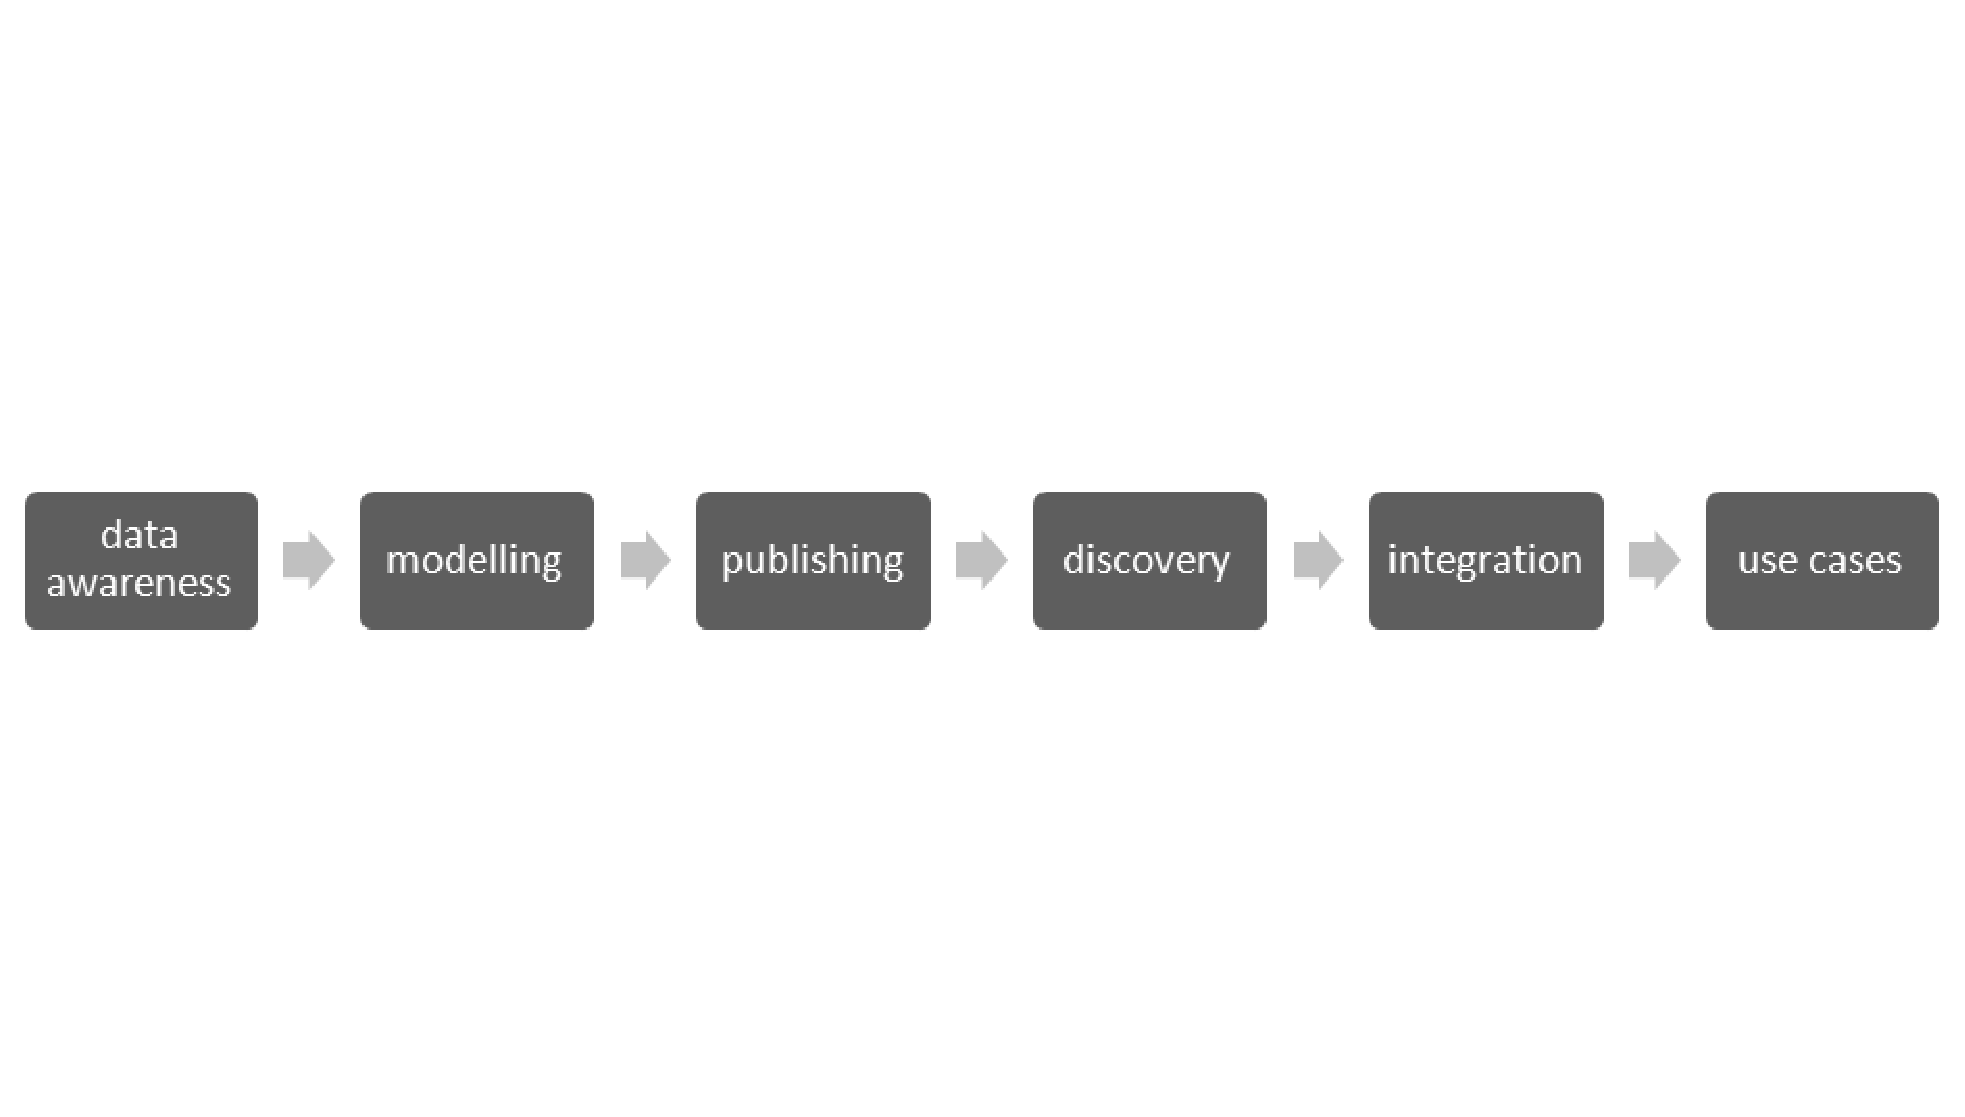
\includegraphics[width=14cm]{images/phd/Hausenblas}
\caption{\textit{Linked Data Lifecycle by M. Hausenblas}.}
\label{fig:hausenblas}
\end{figure}

\begin{figure}[!htb]
\centering
	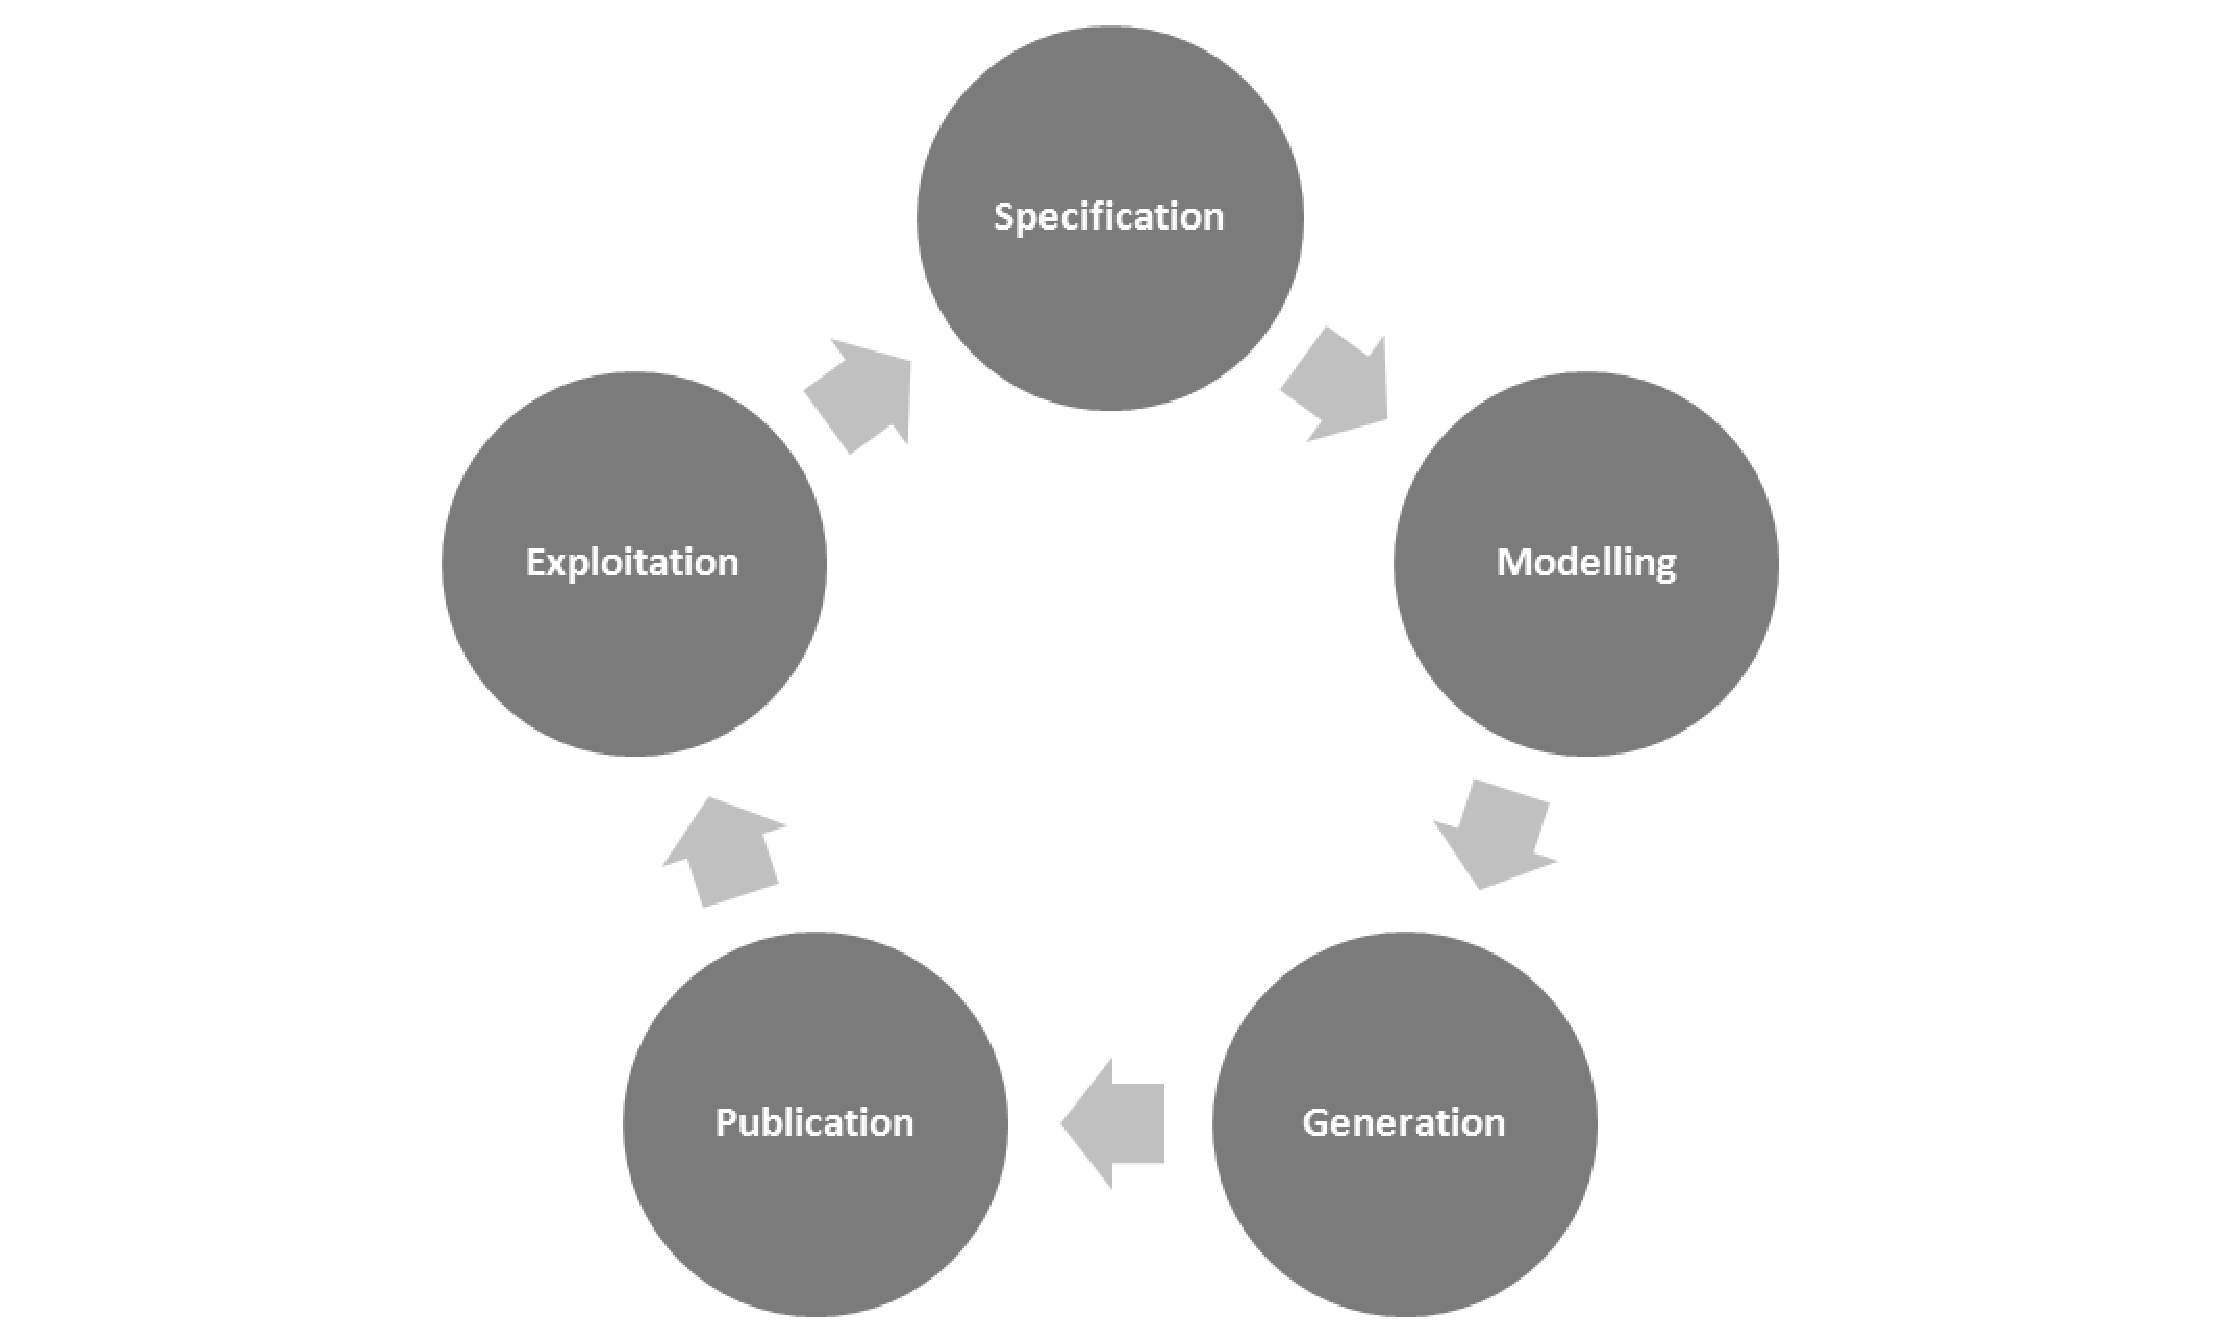
\includegraphics[width=14cm]{images/phd/Villazon-terrazas}
\caption{\textit{Linked Data Lifecycle by B. Villazón-Terrazas}.}
\label{fig:boris}
\end{figure}

En todos ellos se recogen en grandes procesos los pasos a seguir para desplegar el modelo de \linkeddata en una organización. Aunque
existan cambios en la denominación, en el nivel de abstracción o en el orden de algunos procesos, el objetivo coincide en todos ellos. No obstante, estos modelos han surgido, probablemente,
de la experiencia propia de los autores y aún estando en su etapa de desarrollo suponen un avance para afrontar la implantación
de \linkeddata como un proceso de ingeniería cuantificable.

\begin{figure}[!htb]
\centering
	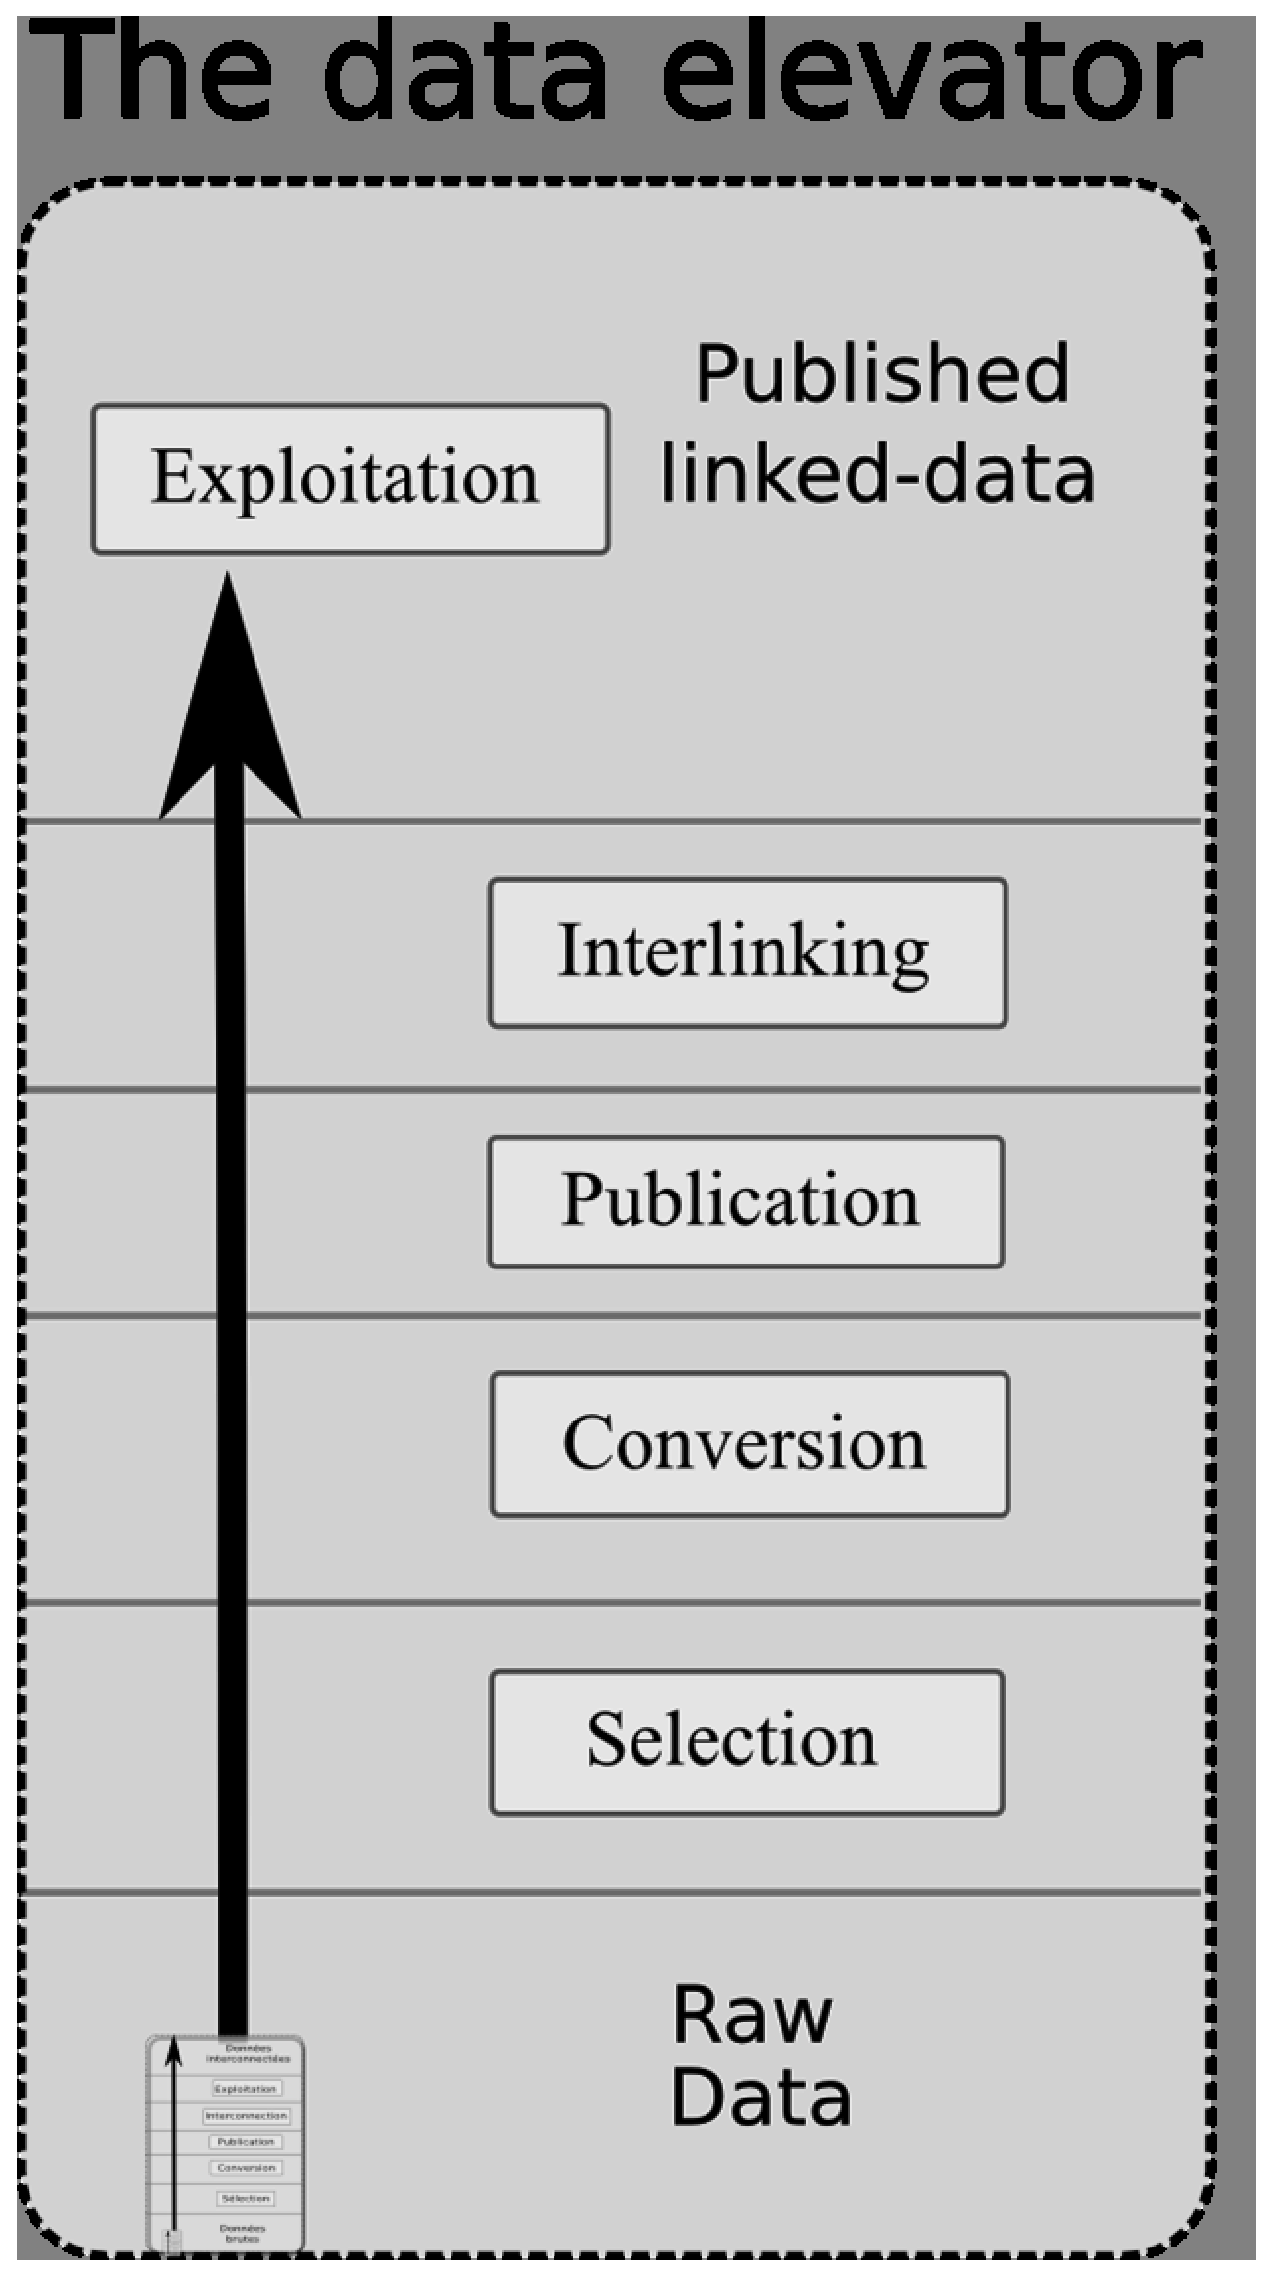
\includegraphics[width=6cm]{images/phd/Data_elevator}
\caption{\textit{DataLift Vision}.}
\label{fig:datalift}
\end{figure}

\clearpage

\subsubsection{\textit{Publishing Open Government Data} del W3C}
Se trata de un borrador de trabajo~\cite{publishing-ogd} (\textit{W3C Working Draft 8 September 2009}) del grupo del \gls{W3C} \textit{\gls{eGovernment} Interest Group} en el cual
se hace una descripción somera sobre cómo publicar datos gubernamentales en la web. Reseñan fundamentalmente una serie de pasos 
para publicar datos sin grandes restricciones y de forma ágil, basándose en 3 pasos,
 ver Tabla~\ref{table:publish-ogd}, de carácter general pero que pueden servir especialmente a perfiles
no técnicos presentes en las instituciones públicas.

\begin{longtable}[c]{|l|p{6.5cm}|p{7.5cm}|} 
\hline
  \textbf{ID} & \textbf{Paso} & \textbf{Descripción} \\\hline
\endhead
  1 &  \textit{Step 1} & \textit{The quickest and easiest way to make data available on the Internet is to publish the data in its raw form.}\\ \hline
  2 &  \textit{Step 2} & \textit{Create an online catalog of the raw data (complete with documentation) so people can discover what has been posted.} \\ \hline
  3 &  \textit{Step 3} &   \textit{Make the data both human- and machine-readable.} \\ \hline
\hline
\caption{\textit{Straightforward Steps to Publish Government Data.}}\label{table:publish-ogd}\\    
\end{longtable}

De la misma forma, en el propio documento se exponen otros factores a valorar en el momento
de publicación de los datos, en la línea de la iniciativa de \linkeddata. Simplemente se trata
de una guía básica prácticamente de carácter divulgativo.

\subsubsection{\textit{LOD2 Stack}}\label{lod2-project}
Dentro del proyecto europeo LOD2~\cite{lod2-project} con nº de contrato: 257943, con duración desde septiembre de 2010
hasta agosto de 2014 y una financiación de más de $7$ millones euros se está desarrollando
una serie de documentos y tecnología asociada a la iniciativa de \lod con el objetivo de proveer
buenas prácticas y herramientas que den soporte a toda la cadena de producción, publicación y consumo
de datos enlazados en distintos dominios. Uno de los últimos resultados que han conseguido y que
se encuentra en continua evolución es la denominada \textit{LOD2 Stack}~\cite{lod2-stack} que contiene una
serie de herramientas para cada una de las etapas necesarias en la apertura de datos como \linkeddata.

\begin{description}
 \item [\textit{OntoWiki}~\cite{tramp-s-2010-ekaw-demo}.] \textit{OntoWiki is a tool providing support for agile, distributed knowledge engineering scenarios}. 
 \item [\textit{PoolParty}~\cite{poolparty}.] \textit{PoolParty is a thesaurus management system and a SKOS editor for the Semantic Web including text mining and linked data capabilities.}
 \item [\textit{Sig.ma}~\cite{citeulike:8529753}.] \textit{Sig.ma is a tool to explore and leverage the Web of Data.}
 \item [\textit{Comprehensive Knowledge Archive Network (CKAN)~\cite{ckan}}.] \textit{CKAN is a registry or catalogue system for datasets or other ''knowledge'' resources.}
 \item [\textit{D2R Server}~\cite{Bizer_Cyganiak_2006}.] \textit{D2R Server is a tool for publishing relational databases on the Semantic Web. }
 \item [\textit{DBpedia Extraction}~\cite{Bizer:2009:D-C:1640541.1640848}.] \textit{DBpedia is a community effort to extract structured information from Wikipedia and to make this information available on the Web.}
 \item [\textit{DL-Learner}~\cite{lehmann2009}.] \textit{DL-Learner is a tool for supervised Machine Learning in OWL and Description Logics.}
 \item [\textit{MonetDB}~\cite{Boncz06monetdb/xquery:a}.] \textit{MonetDB is an open-source high-performance database system that allows to store relational, XML and RDF data}.
 \item [\textit{SemMF}.] \textit{SemMF is a flexible framework for calculating semantic similarity between objects that are represented as arbitrary RDF graphs.}
 \item [\textit{Silk Framework}~\cite{www2009227}.] \textit{The Silk Linking Framework supports data publishers in setting explicit RDF links between data items within different data sources.}
 \item [\textit{Sindice}~\cite{TummarelloDO07}.] \textit{Sindice is a state of the art infrastructure to process, consolidate and query the Web of Data. }
 \item [\textit{Sparallax}~\cite{Sparallax}.] \textit{Sparallax is a faceted browsing interface for SPARQL endpoints, based on Freebase Parallax.}
 \item [\textit{Triplify}~\cite{Triplify}.] \textit{Triplify provides a building block for the ``semantification'' of Web applications.}
 \item [\textit{OpenLink Virtuoso}~\cite{Virtuoso}.] \textit{Virtuoso is a knowledge store and virtualization platform that transparently integrates Data, Services, and Business Processes across the enterprise.}
 \item [\textit{WIQA}~\cite{wiqa}.] \textit{The Web Information Quality Assessment Framework is a set of software components that empowers information consumers to employ a wide range of different information quality assessment policies to filter information from the Web.} 
\end{description}
% 
% \begin{figure}[!htb]
% \centering
% 	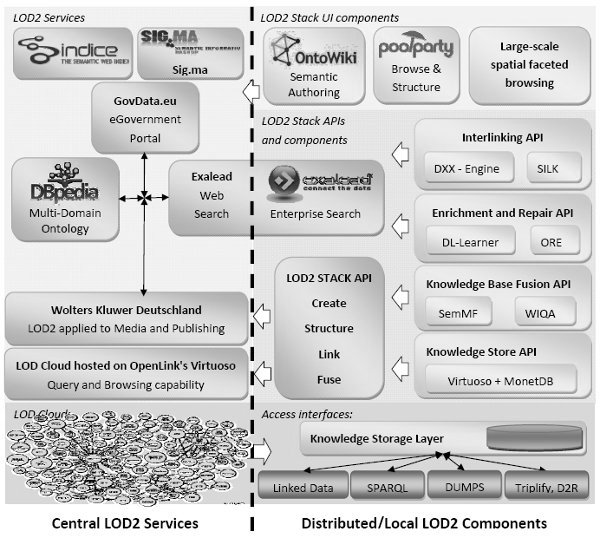
\includegraphics[width=10cm]{images/phd/lod2-high-level-architecture}
% \caption{\textit{LOD2 high-level Architecturel} (extraída del portal del proyecto LOD2).}
% \label{fig:lod-arch}
% \end{figure}


Como se puede observar este grupo de herramientas dan soporte a todo el ciclo de vida de los datos enlazados y proveen
una plataforma genérica en la cual cualquier persona o entidad pueda integrar un nuevo conjunto de datos, desde
recursos ya disponibles en \gls{RDF} hasta documentos de texto. La realización de este proyecto es de una suma transcendencia
para la comunidad, ya que en el despliegue de una infraestructura basada en datos enlazados se suele incurrir en las mismas
dudas y problemas, por lo que disponer de una guía que parta desde un punto de vista teórico hasta su realización práctica, 
supone un gran avance respecto a las especificaciones teóricas, recetas y buenas prácticas que se han mencionado en las
secciones anteriores. 

Por otra parte, las herramientas desarrolladas se encuentran enclavadas dentro de un proceso o ciclo de vida de datos enlazados,
ver Figura~\ref{fig:lod-lifecycle}. Se trata de un modelo iterativo y realimentado, en el que se completan las distintas fases
para cumplir con la producción, publicación y consumo de datos, utilizando las herramientas previamente comentadas y atacando
las principales barreras que se suelen encontrar, así como aplicando los principios de diseño de \linkeddata.

\begin{figure}[!htb]
\centering
	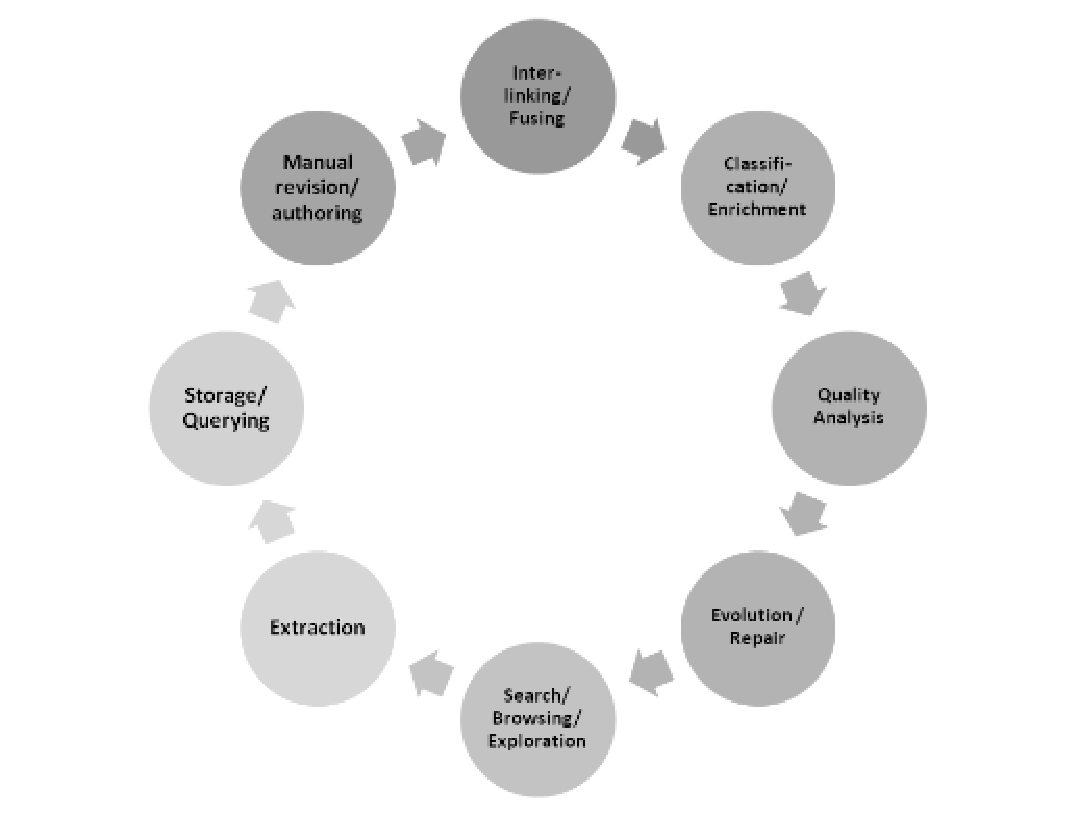
\includegraphics[width=12cm]{images/phd/lod-lifecycle-small}
\caption{\textit{Linked Data LifeCycle} (extraída de LOD2 Demo).}
\label{fig:lod-lifecycle}
\end{figure}

Para la aplicación de los principios de \linkeddata es realmente conveniente prestar atención al trabajo
desarrollado en este proyecto, no obstante, teniendo en cuenta que tan sólo se cuenta con un año de desarrollo
es complicado aplicar su enfoque de forma integral.

\subsubsection{\textit{Toward a Basic Profile for Linked Data} de IBM}
Dentro de la actividad de IBM en el campo de \linkeddata, se ha identificado
la necesidad de fijar una serie de reglas para aplicar esta iniciativa de forma
cuantificable. El objetivo de esta guía es llegar a introducir dentro de una herramienta
como \textit{Rationale} (también perteneciente a IBM) el modelo arquitectónico propuesto por los datos
enlazados, cumpliendo las directrices de la misma con la meta de obtener
la tecnología necesaria que sirva para integrar datos de forma ágil en las aplicaciones.

El término utilizado por IBM es \textit{Basic Profile Resources}~\cite{basic-profile-ibm} que se define como recursos \linkeddata accesibles mediante HTTP que siguen una serie de patrones
y convenciones comunes. En general, estos recursos dependen del dominio en el cual
estén definidos y tan sólo se delimitan como comunes algunos considerados transversales a cualquier dominio. Estos recursos siguen una serie de reglas, ver Tabla~\ref{table:basic-ibm}, y reutilizan
vocabularios existentes con el objetivo de cumplir con la iniciativa de \linkeddata. 

\begin{longtable}[c]{|l|p{6.5cm}|p{7.5cm}|} 
\hline
  \textbf{ID} & \textbf{Rule} & \textbf{Descripción} \\\hline
\endhead
  1 &  \textit{Basic Profile Resources are \gls{HTTP} resources} & \textit{They can be created, modified, deleted and read using standard HTTP methods.}\\ \hline
  2 &  \textit{Basic Profile Resources use \gls{RDF} to define their states} & \textit{The state of a Basic Profile Resource (in the sense of state used in the REST architecture) is defined by a set of RDF triples.} \\ \hline
  3 &  \textit{You can request an RDF/XML representation of any Basic Profile Resource} &   \textit{The resource might have other representations.} \\ \hline
  4 &  \textit{Basic Profile clients use Optimistic Collision Detection during update} &   \textit{Because the update process involves getting a resource first, and then modifying it and later putting it back on the server, there is the possibility of a conflict (for example, another client might have updated the resource since the GET action). To mitigate this problem, Basic Profile implementations should use the HTTP If-Match header and HTTP ETags to detect collisions.} \\ \hline
  5 &  \textit{Basic Profile Resources use standard media types} &   \textit{ Basic Profile does not require and does not encourage the definition of any new media types.} \\ \hline
  6 &  \textit{Basic Profile Resources use standard vocabularies} &   \textit{Basic Profile Resources use common vocabularies (classes, properties, and so forth) for common concepts.} \\ \hline
  7 &  \textit{Basic Profile Resources set \texttt{rdf:type} explicitly.} &   \textit{A resource's membership in a class extent can be derived implicitly or indicated explicitly by a triple in the resource representation.} \\ \hline
  8 &  \textit{Basic Profile Resources use a restricted number of standard data types} &   \textit{RDF does not define data types to be used for property values, so Basic Profile lists a set of standard datatypes to be used in Basic Profile.} \\ \hline
  9 &  \textit{Basic Profile clients expect to encounter unknown properties and content} &   \textit{Basic Profile provides mechanisms for clients to discover lists of expected properties for resources for particular purposes.} \\ \hline
  10 &  \textit{Basic Profile clients do not assume the type of a resource at the end of a link} &   \textit{Many specifications and most traditional applications have a "closed model," by which we mean that any reference from a resource in the specification or application necessarily identifies a resource in the same specification.} \\ \hline
  11 &  \textit{Basic Profile servers implement simple validations for Create and Update} &   \textit{Basic Profile servers should try to make it easy for programmatic clients to create and update resources.} \\ \hline
  12 &  \textit{Basic Profile Resources always use simple RDF predicates to represent links} &   \textit{Basic Profile makes it very simple to know how links will appear in representations and also makes it very simple to query them.} \\ \hline
\hline
\caption{\textit{Basic Profile Resources.}}\label{table:basic-ibm}\\    
\end{longtable}

Repasando esta lista de reglas se puede observar como algunas afectan a los principios $2º$ y $3º$ de \linkeddata sin
modificar su significado pero especificando de forma más concreta el funcionamiento esperado. La importancia
de este reciente artículo reside en varios puntos: es realizado por IBM, es coherente con las reglas de \linkeddata y
ofrece un carácter práctico desde el punto de vista de la ingeniería para implementar, o en este caso, incluir
la arquitectura y modelo de trabajo de datos enlazados en una plataforma existente como es \textit{Rationale}.


\subsubsection{Metodología y Proceso de Adopción de \linkeddata en la Biblioteca del Congreso de Chile}
En este trabajo se propone una metodología~\cite{DBLP:conf/i-semantics/Cifuentes-SilvaSG11,methodologyCaepia2011} y proceso de adopción de la iniciativa de \linkeddata en el contexto
de las Administraciones Públicas y concretamente en la Biblioteca del Congreso de Chile para la publicación
de la legislación actual e histórica. En general, se trata en realidad de la especificación de una infraestructura
para dar soporte a los datos enlazados y un proceso de generación con diferentes etapas, que parten de un
caso particular motivador pero que se podrían aplicar a un contexto genérico. Una de las diferencias respecto 
al proyecto LOD2 reside en las herramientas seleccionadas para llevar a cabo los distintos procesos de producción, publicación y consumo de datos enlazados y por otra parte la
adición de servicios de consumo de datos especialmente dirigidos a los usuarios de la Administración, como es la visualización
de las normas.

También, hay que destacar el proceso de adopción definido en este enfoque, ver Figura~\ref{fig:bcn-proceso}, en el cual
quedan recogidos los pasos para promocionar las bases de datos legislativas utilizando datos enlazados. Este proceso
es similar al propuesto por el \gls{W3C}, ver Sección~\ref{linked-data-cookbook}, y ciclo de vida definido en el proyecto LOD2, ver Figura~\ref{fig:lod-lifecycle}, sin embargo 
difiere en el nombrado de los procesos y las herramientas a utilizar en cada una de las fases.

\begin{figure}[!htb]
\centering
	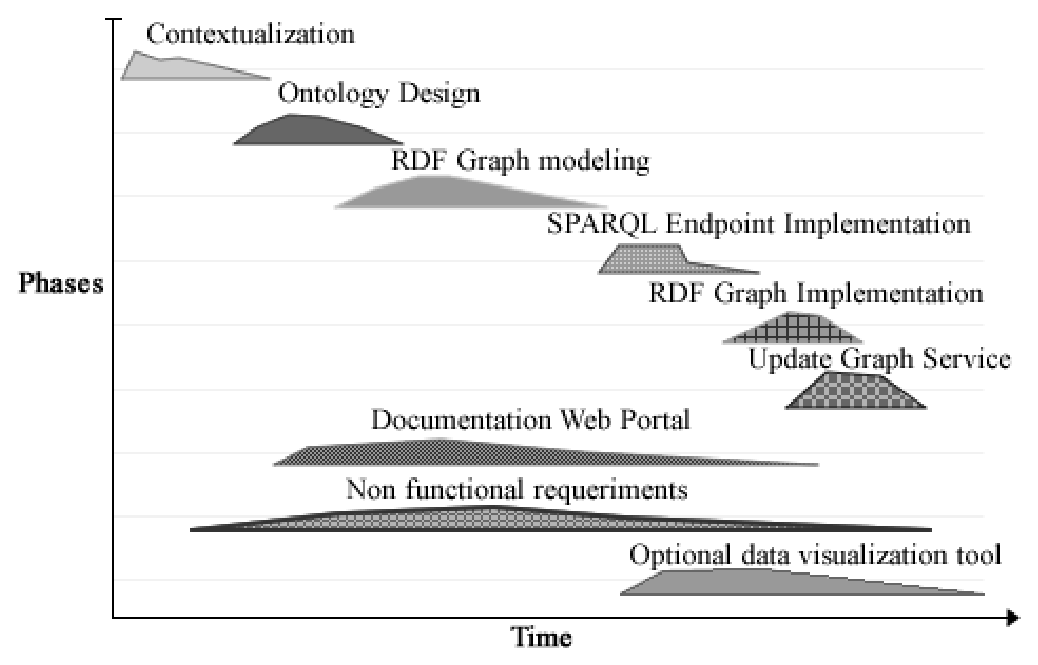
\includegraphics[width=10cm]{images/phd/process}
\caption{Proceso de implantación de \linkeddata en la Biblioteca del Congreso de Chile.}
\label{fig:bcn-proceso}
\end{figure}


% \begin{figure}[!htb]
% \centering
% 	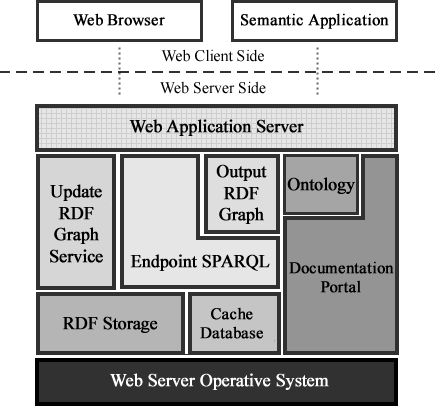
\includegraphics[width=10cm]{images/phd/infrastructure}
% \caption{Infraestructra \linkeddata propuesta en la Biblioteca del Congreso de Chile.}
% \label{fig:bcn-infraestructura}
% \end{figure}

\subsubsection{\textit{Talis Platform}}
En este caso la plataforma Talis~\cite{talis} es un servicio o producto que sirve para la creación de una
infraestructura de \linkeddata en la nube. Ha tenido un gran éxito ya que sus creadores son grandes
impulsores de la iniciativa (por ejemplo son los autores de \textit{Linked Data Patterns}) y han trabajado
en casos de enorme repercusión, como la apertura de datos públicos del Gobierno del Reino Unido. Ofrecen 
 una \textit{suite} de herramientas y servicios para cumplir las directrices de \linkeddata, teniendo en cuenta 
la mayor parte de la casuística presente en la producción, publicación y consumo de datos enlazados. En resumen, se provee una plataforma
que cubre toda la cadena de valor de los datos enlazados y cumple todas las directrices necesarias.

Entre las características más llamativas que ofrecen dentro de esta plataforma se encuentran las
siguientes (extraídas de la propia página web de Talis):

\begin{itemize}
    \item \textit{A simple, consistent web API for storing, managing and retrieving both structured and unstructured data.}
    \item \textit{Flexible, schema-free metadata that allows applications to be easily evolved.}
    \item \textit{A range of data access and query options enabling easy integration into both new and existing applications.}
    \item \textit{Access control options to support hosting of both public and private data.}
    \item \textit{A data hosting solution that is founded on open internet standards and web architectural best practices.}
    \item \textit{Software as a Service, enabling rapid development with zero deployment costs.}
    \item \textit{Low, even free, utility based pricing for services and hosting allowing costs to grow with usage.}
    \item \textit{A highly available and scalable infrastructure to ensure that the repository grows in line with your applications needs.}
\end{itemize}

Evidentemente este tipo de soluciones son de extraordinario interés para las Administraciones Públicas, ya que consiguen
un producto llave en mano con todas las capacidades necesarias para disponer de una infraestructura de datos
enlazados de última generación. Es interesante destacar esta plataforma por dos motivos principales: sus creadores
son relevantes desde un punto de vista científico y han realizado una gran transferencia tecnológica desde
el campo de la investigación al industrial.

En la misma línea de la plataforma Talis se encuentran otras empresas que ofrecen productos y herramientas
de alto valor como son Virtuoso de OpenLink o ToqQuadrant. Todos ellos son miembros activos en la comunidad
de \linkeddata y están presentes en los principales grupos de trabajo de esta iniciativa en el \gls{W3C}.
 
\subsubsection{\textit{Linked Open Data: The Essentials}}\label{linked-data-spec}
Este libro~\cite{Bauer2012} realizado en colaboración entre \gls{REEEP} (\textit{Renewable Energy and Energy Efficiency Partnership}) y la compañía \textit{Semantic Web}
es un manual que da respuesta a algunas de las preguntas comunes que surgen en el despliegue de una infraestructura de datos enlazados
en el seno de una organización. En general, se trata de una recopilación de las buenas prácticas que se han revisado
en los anteriores apartados y que focaliza en los beneficios de la publicación de datos enlazados para las
organizaciones. La parte más destacada de este libro, ver Figura~\ref{fig:lod-essentials}, se centra en la descripción de las tareas
a realizar y de los posibles servicios haciendo hincapié en las tareas de publicación y consumo de datos enlazados.

\begin{figure}[!htb]
\centering
	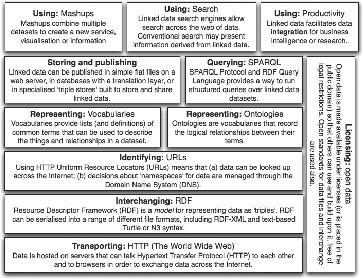
\includegraphics[width=10cm]{images/phd/lod-essentials}
\caption{\textit{Elementos of the Linked Open Data Puzzle}.}
\label{fig:lod-essentials}
\end{figure}


\subsubsection{Documentación específica}\label{linked-data-spec}
Desde distintas organizaciones tales como Administraciones Públicas y Universidades,
así como personalidades relevantes en esta materia se ha promovido la realización de proyectos, guías y artículos que tratan diversos aspectos
relacionados con la iniciativa de \linkeddata. Todos ellos tratan de aportar nuevos enfoques, herramientas y documentación
a los distintos procesos implicados en el despliegue de esta iniciativa, entre los que pueden destacarse:

\begin{itemize}
 \item ``\textit{A Proposal for Governmental Data URIs}'' realizado por Gregory Todd Williams, Tim Lebo y Alvaro Graves.  % http://iw.rpi.edu/wiki/A_Proposal_for_Governmental_Data_URIs
 \item ``\textit{Designing \gls{URI} Sets for the UK Public Sector}''~\cite{uris-uk} realizado por ``The Cabinet Office'' del Reino Unido. 
 \item ``\textit{Federal Information Security Management Act (FISMA)}'' proyecto realizado por  el ``National Institute of Standards and Technology'' de Estados Unidos.
 \item La documentación disponible en la Biblioteca del Congreso de Estados Unidos.
 \item Los artículos de Jeni Tennison sobre distintos aspectos relativos al diseño de URIs, etc.
 \item El \textit{framework} SERIMI~\cite{Serimi} de reconciliación de entidades.
 \item Los documentos y software elaborados por la empresa Epimorphics.
 \item Las guías de datos abiertos y enlazados de las distintas Administraciones Públicas, tanto a nivel estatal: 
España, Reino Unido, Francia, Alemania, etc., como a nivel regional: Asturias, País Vasco o Cataluña o incluso local como
en el Ayuntamiento de Zaragoza.
\end{itemize}

En general se trata de documentos o herramientas que nacen de la necesidad y experiencia en la resolución de ciertos
 problemas relacionados con la apertura de datos y su enlazado, que se reproducen en cada escenario en el cual se
aplica esta iniciativa. Todo este trabajo y esfuerzo supone un gran valor para la comunidad de desarrolladores
y de personas implicadas en la aplicación de estos principios.

\subsection{Escenarios y Casos de Uso de Éxito}
La irrupción de la corriente de \linkeddata ha conllevado la realización práctica y real de una parte de la denostada Web
Semántica. Muchas son las instituciones, administraciones públicas,
empresas privadas, universidades, hospitales, etc., que bajo esta corriente están
liberando sus datos en el entorno web siguiendo las directrices  marcadas por
\textit{Tim Berners-Lee}. El principal objetivo consiste en la apertura de datos, para que
una vez publicados sirvan como fuente para la creación de aplicaciones agregando
distintos recursos (\textit{mashups}), facilitando la transparencia de comportamiento en
ciertos organismos, suministrando servicios de valor añadido basados en el contexto
del usuario o simplemente desde un punto de vista de tendencia, para obtener
presencia en la nueva \wod. 

No obstante, este nuevo enfoque conlleva varios desafíos a nivel científico que están siendo
abordados actualmente, tales como el procesamiento de grandes cantidades de
datos de forma eficiente, gestión-formalización-explotación del conocimiento
subyacente mediante reglas, razonamiento distribuido, \textit{stream-reasoning}, \textit{real
time linked data}, \textit{complex event processing}, reconciliación de entidades,
visualización etc., los casos de uso de aplicación de estas investigaciones representan un abanico muy amplio: recomendación de recursos
(películas, libros, etc.), análisis de sentimientos y opiniones, domótica,
\textit{smart-cities}, computación ubicua, \textit{green computing}, sistemas de soporte a la
decisión en campos como \textit{e-Health}, etc.

Hasta el momento esta iniciativa ha estado muy ligada al mundo técnico, es decir, tanto la publicación como el 
consumo de los datos estaba muy orientado a un perfil fundamentalmente técnico. No obstante, al igual que con la web que hoy conocemos, 
la \wod todavía no trascendido al gran público, es por ello que surgen varios desafíos~\cite{DBLP:journals/semweb/DadzieR11} para 
conseguir el despegue definitivo de esta corriente:

\begin{enumerate}
 \item Necesidad de una capa de presentación. Si una persona buscara cierto recurso 
 que tiene definido según unas necesidades, la expresión de esta consulta implicaría características de 
sistemas de \textit{Information Retrieval} o tareas de análisis de sentimientos. Concretamente: a) descubrimiento de qué fuentes pueden tener 
disponible esa información; b) validación y cooperación entre las distintas fuentes de datos disponibles; c) consulta a 
las fuentes de datos seleccionadas y d) análisis, presentación y manejo de las vistas de los resultados. En este sentido, la tendencia actual 
reside en ``ocultar'' la existencia de varios datasets detrás de los sistemas de búsqueda, así como la consulta y manejo de los 
resultados, de tal manera que el usuario no es consciente de las oportunidades de explotación de datos de las que podría disponer. 
Es necesario aclarar que el conocimiento de la tecnología no debe ser la clave para la explotación de la misma por el usuario 
final, pero si que es necesario proveer los métodos y herramientas adecuadas para que el usuario obtenga el máximo partido de 
la información subyacente. De esta manera si la tendencia de \linkeddata supone una revolución respecto a la actual web de documentos, se 
deberían proveer nuevos mecanismos de acceso a la información y no restringirse a los tradicionales modelos de interacción con el 
usuario (por ejemplo un formulario de búsqueda). 
\item Combinación efectiva de los distintos \datasets. Teniendo en cuenta que existe un catálogo de datos y 
  vocabularios en constante crecimiento, es necesario proveer los mecanismos necesarios (alineación, \textit{mapeo} y fusión) para que 
la combinación de los mismos sea eficiente de modo que la identificación de recursos similares, el 
encaje mediante propiedades o la mezcla de recursos sea intuitiva, tanto desde un punto de vista técnico como del usuario final. 
Las técnicas que permiten llevar a cabo este desafío no son deterministas y en muchos casos se basan en algoritmos que chequean 
la estructura de los recursos, o bien realizan comparaciones basadas en procesamiento del lenguaje natural entre las descripciones de los recursos.
\end{enumerate}

En el contexto de \linkeddata se manifiestan dos principales vías de actuación sobre los datos: publicación y consumo, concretamente en el campo de consumo de 
datos surgen varios interrogantes como:
\begin{itemize}
\item Gestión de datos a nivel web.
\item Procesamiento de consultas federadas~\cite{sparqlOpt}.
\item Búsqueda.
\item Descubrimiento de \datasets y recursos: URIs, datos adicionales o datasets relevantes para una consulta.
\item \textit{Datasets} evolutivos: cómo afectan los cambios en los datasets a las consultas, monitorización.
\item Razonamiento e inferencia de conocimiento en la \wod.
\item Calidad de los datos: evaluación de la calidad de la información, confianza y \textit{provenance}.
\item Interfaz de Usuario para la interacción con la \wod: interacción y usabilidad, visualización, interfaces basadas en lenguaje natural.
\end{itemize}


Por otra parte, tanto en las Administraciones Públicas como en otros dominios 
se está trabajando exhaustivamente en el campo de la reutilización de datos y servicios basados en semántica, en la actualidad 
se pueden señalar algunos ejemplos:
\begin{itemize}
\item Gestión de bibliotecas digitales~\cite{DBLP:journals/chb/Garcia-CrespoBPS11}, la Biblioteca del Congreso de Chile o del Congreso de Estados Unidos.
\item Sistemas de búsqueda y recomendación basados en perfiles de usuario enlazados~\cite{DBLP:conf/www/LatifAHTM10}.
\item Sistemas para el soporte a la decisión~\cite{DBLP:journals/ijdsst/Garcia-ManotasLSV10}, especialmente en el dominio de \textit{e-Health}.
\item Gestión, publicación y servicios sobre información financiera~\cite{DBLP:journals/eswa/Esteban-GilSVF12,DBLP:conf/iwinac/GomezSVTM09}.
\item Otros múltiples campos de actuación:  \gls{GIS}+\linkeddata, turismo, tráfico, educación, domótica, \textit{semantic sensors}, etc.
\end{itemize}

En último término todas las iniciativas basadas en \linkeddata convergen al objetivo principal de la misma:
\begin{Frame}
\textit{Linked Data is about using the Web to connect related data that wasn't previously linked, or using the Web to lower the barriers 
to linking data currently linked using other methods.} 
\end{Frame}


Teniendo en cuenta el valor añadido de la visualización de datos para Linked Data,
 se pueden establecer una serie de requisitos~\cite{journals/semweb/DadzieR11} a cumplir, que actualmente están parcialmente cubiertos 
por algunas herramientas, no obstante, se puede establecer una guía de características necesarias para el manejo de datos enlazados y su 
visualización, siendo uno de los grandes elementos de investigación actual.
\begin{itemize}
 \item Requisitos de alto nivel: a) capacidad para generar vistas agregadas de los datos; b) soporte para la creación de filtros y c) soporte para 
la visualización detallada de los recursos.
\item  Requisitos de consumo de datos: a) manejo de datos multidimensionales; b) manejo de datos jerárquicos;c) generación de estructuras de representación: grafos, árboles, etc.; d) identificación de las relaciones significativas en los datos;
e) extracción de datos y nuevas relaciones y f) contextualización de usuario y multidispositivo.
\item Requisitos directamente relacionados con \linkeddata: a) navegación entre los distintos datasets; b) exploración de los datos 
para obtener consciencia de la estructura y de las relaciones; \linebreak c) exploración que permita análisis con el objetivo de identificar incoherencias, etc.;
d) consulta transversal a través de los distintos datasets mediante un lenguaje formal y e) capacidad para extraer partes de los datos para su posterior reutilización.
\item Requisitos relacionados con la navegación semántica: a) navegación facetada y contextualizada del usuario; b) exploración del conocimiento, inferencia, etc.;
c) consulta avanzada con filtros de lenguaje natural; d) análisis detallado y explicación de las inferencias y e) presentación de resultados de análisis.
\end{itemize}




